\chapter{Esperimenti e risultati}
\label{chap:esperimenti}
In questo capitolo si descrivono gli esperimenti effettuati.
Nel~\Cref{sec:exp:dataset} si descrivono gli algoritmi utilizzati per generare i \emph{dataset} sintetici, le caratteristiche dei \emph{dataset} di terze parti e le metriche utilizzate per valutare la difficoltà di classificazione di un dataset;
nel~\Cref{sec:impostazione_esperimenti} si descrivono le strategie utilizzate per effettuare gli esperimenti e si descrivono le caratteristiche comuni, come il criterio di selezione dei migliori modelli e l'ambiente di esecuzione;
nel~\Cref{sec:exp:synth_2d} si descrivono gli esperimenti effettuati su \emph{dataset} sintetici a due dimensioni;
nel~\Cref{sec:exp:synth_3d} si descrivono gli esperimenti effettuati su \emph{dataset} sintetici a 3 dimensioni;
nel~\Cref{sec:exp:real_ds} si descrivono gli esperimenti effettuati su alcuni \emph{dataset} di terze parti;
nel~\Cref{sec:comparazione_metodi} si confrontano i risultati ottenuti con l'approccio \emph{budgeted SVC} con alcune implementazioni di algoritmi presenti in letteratura e descritti nel~\Cref{chap:sparse_svc}; per concludere, nel~\Cref{sec:memorizzazione_compressa} si descrive un metodo per memorizzare i modelli in un formato compresso, riducendo i requisiti di spazio. 

\section{Dataset}\label{sec:exp:dataset}
Per gli esperimenti descritti in questo capitolo sono state usate due tipologie di dataset. 
La prima categoria è composta da \emph{dataset} sintetici, generati specificatamente per questo lavoro, mentre la seconda categoria è composta da alcuni \emph{dataset} di terze parti utilizzati in letteratura. 
Le due tipologie presentano vantaggi e svantaggi. Nel primo caso risulta molto comodo poter modificare a piacimento le caratteristiche dei dataset, per esempio per valutare algoritmi su \emph{dataset} di difficoltà crescente, oppure con quantità di rumore crescente.
Lo svantaggio è che si potrebbero ottenere dei risultati poco significativi, perché ottenuti su dati generati \emph{ad hoc} e poco confrontabili con altri modelli. 
Per questo motivo ha senso utilizzare anche dei \emph{dataset} di terze parti, spesso utilizzati anche da altri lavori presenti in letteratura.

\subsubsection{Metriche delle difficoltà di un dataset}\label{sec:metriche_dataset}
Per avere a priori un'indicazione della difficoltà dei \emph{dataset} sintetici, intesa come difficoltà nel trovare una superficie di separazione soddisfacente, sono state considerate alcune metriche, in particolare F1 e F1v~\cite{ds_complexity}, descritte brevemente nell'elenco seguente.
\begin{itemize}
    \item \textbf{F1} è la sigla per la metrica \emph{Maximum Fisher’s discriminant ratio}. Questa metrica misura la sovrapposizione tra i vari attributi per ogni classe.
    % La metrica è calcolata come
    % \begin{equation*}
    %     F1=\frac{1}{1+\max_{j=1}^{d}r_{f_{j}}},
    % \end{equation*}
    % dove $r_{f_{j}}$ è il \emph{discriminant ratio} per l'attributo $j$.
    Il valore di F1 è compreso nell'intervallo $(0,1]$. Più il valore è vicino a uno, più il \emph{dataset} è difficilmente classificabile, perché non esistono attributi in grado di separare le due classi. Al contrario, un valore vicino a zero indica la presenza di un attributo $f$ per cui esiste una superficie di separazione perpendicolare all'asse di $f$ in grado di separare equamente le classi delle etichette.
    \item \textbf{F1v} è la sigla per la metrica \emph{Directional-vector Maximum Fisher’s Discriminant Ratio}. Quantifica quanto separabili siano due classi una volta proiettate su un vettore scelto per rendere i dati separabili.
    Anche il valore di F1v è compreso nell'intervallo $(0,1]$ e valori vicini a zero indicano dati facilmente separabili.    
    Si rimanda a~\cite{ds_complexity} per la definizione completa di F1v.
\end{itemize}

Dal punto di vista pratico, queste metriche sono state calcolate per ogni \emph{dataset} utilizzando la libreria python problexity~\cite{problexity} in versione 0.5.6.


\subsection{Dataset sintetici}
I \emph{dataset} sintetici sono costruiti selezionando dei punti generati casualmente e in seguito etichettati da una funzione.
Per decidere l'etichetta di un punto sono state utilizzate due tipologie di funzioni: una funzione sinusoidale e una funzione paraboloide.
\begin{itemize}
    \item \textbf{Funzione sinusoidale} Fissando i parametri $\beta,\rho,\theta$, per un vettore $\Vec{x}=[x^{(1)},x^{(2)}]$, $\Vec{x} \in R^2$, l'etichetta $y$ è calcolata con la funzione
    \begin{equation}\label{eq:sinusoid_dataset_lf}
    \textrm{lf}(\Vec{x}) = \sign\left(\frac{1}{(1 + \exp(-\beta(x^{(1)} - 0.5)) + \rho \sin(2\pi\theta x^{(1)})} - x^{(2)}\right).
    \end{equation}
    Questa funzione di etichettatura è utilizzata solo per dati con due attributi. La~\Cref{fig:sinusoid_dataset} mostra alcuni esempi di \emph{dataset} e funzioni di etichettatura al variare dei parametri.

    \item \textbf{Funzione paraboloide} Fissati i parametri $\alpha, x_\text{shift}, y_\text{shift}$, per un vettore $\Vec{x}=[x^{(1)}\dots, x^{(d)}]$, $\Vec{x} \in \mathrm{R}^d$, l'etichetta $y$ è calcolata con la funzione
    \begin{equation}\label{eq:pacman_dataset_lf}
    \textrm{lf}(\Vec{x})= x^{(d)} - \sum_{j=1}^{d-1}\alpha(x^{(j)} - x_\text{shift})^2 - y_\text{shift}.
    \end{equation}
    Il parametro $\alpha$ controlla l'ampiezza del paraboloide, mentre $x_\text{shift}$ e $y_\text{shift}$ traslano il vertice del paraboloide.
    La~\Cref{fig:pacman_dataset} mostra alcuni esempi di \emph{dataset} e funzioni di etichettatura al variare dei parametri.
\end{itemize}
\begin{figure}
    \centering
    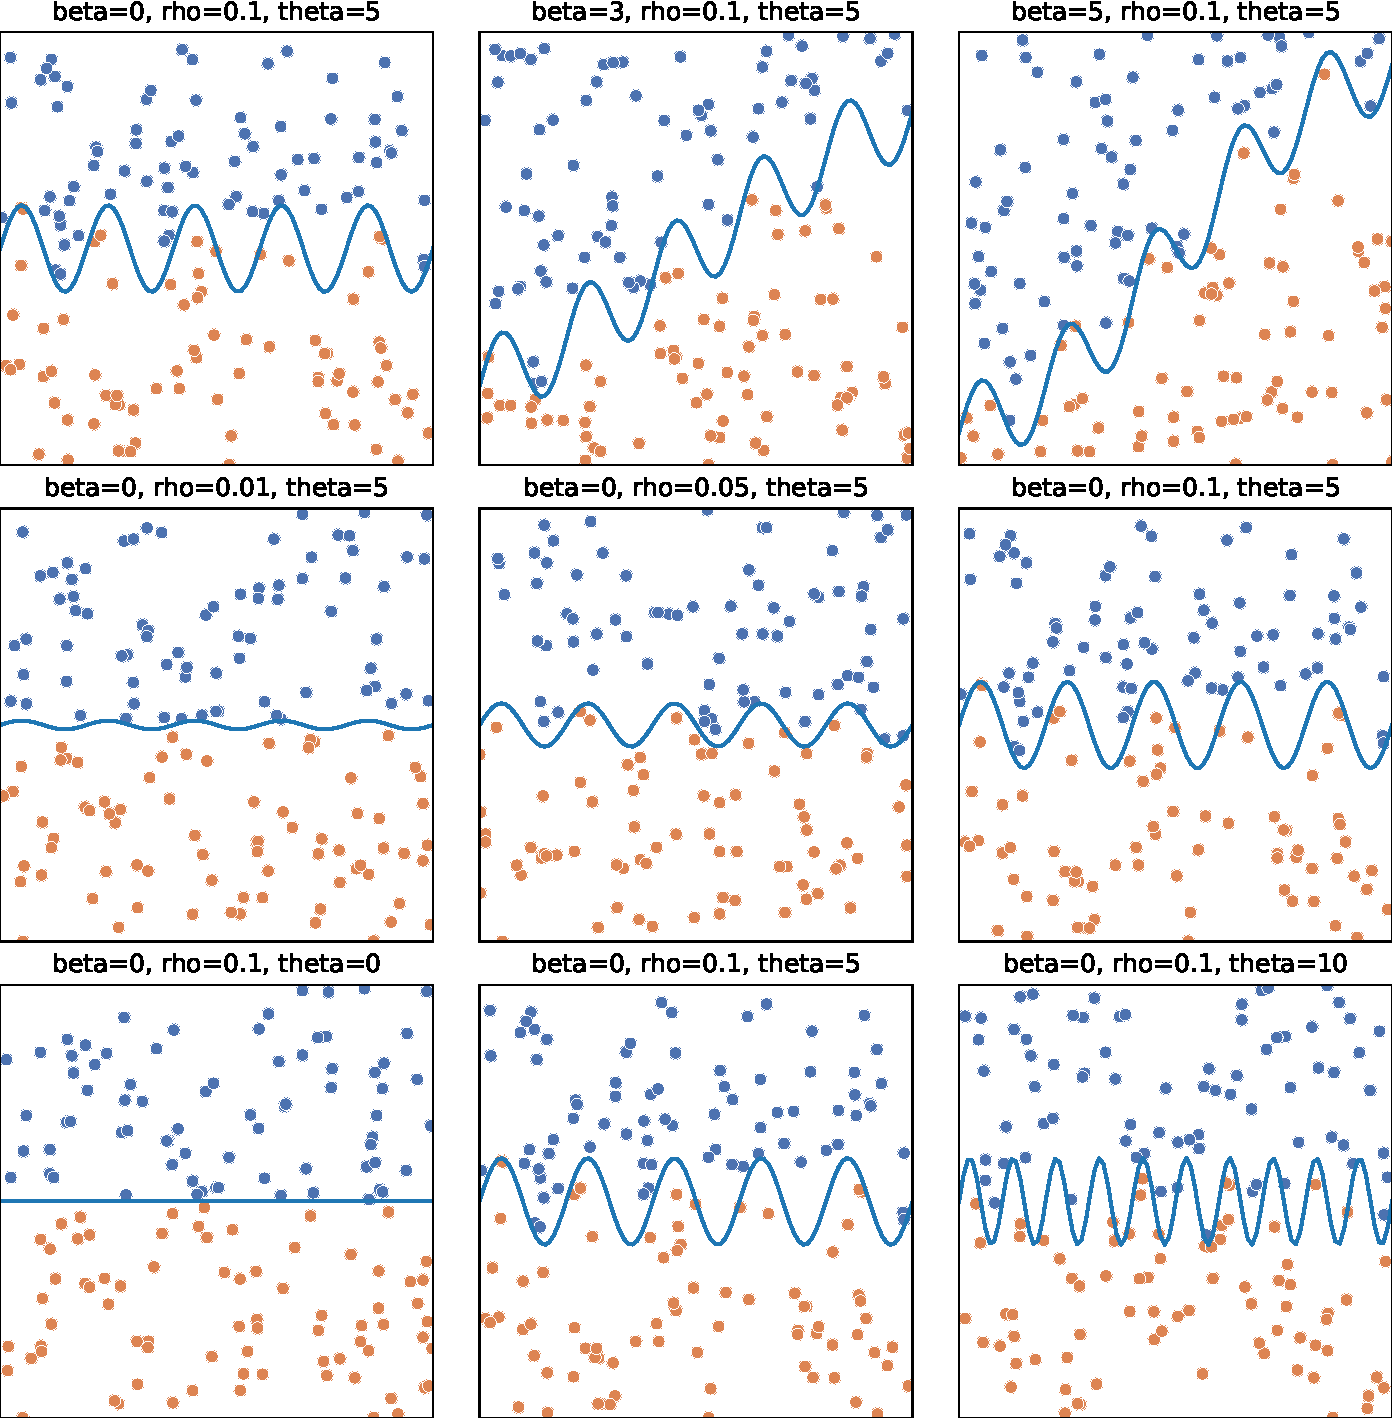
\includegraphics[width=.7\linewidth]{img/sinusoid_dataset_param_influence.pdf}
    \caption[Esempio di \emph{dataset} sintetici generati con funzione sinusoidale.]{Esempio di \emph{dataset} sintetici generati con funzione sinusoidale. 
    $\beta$ controlla l'inclinazione, $\rho$ controlla l'ampiezza, $\theta$ la frequenza.}
    \label{fig:sinusoid_dataset}
\end{figure}
\begin{figure}
    \centering
    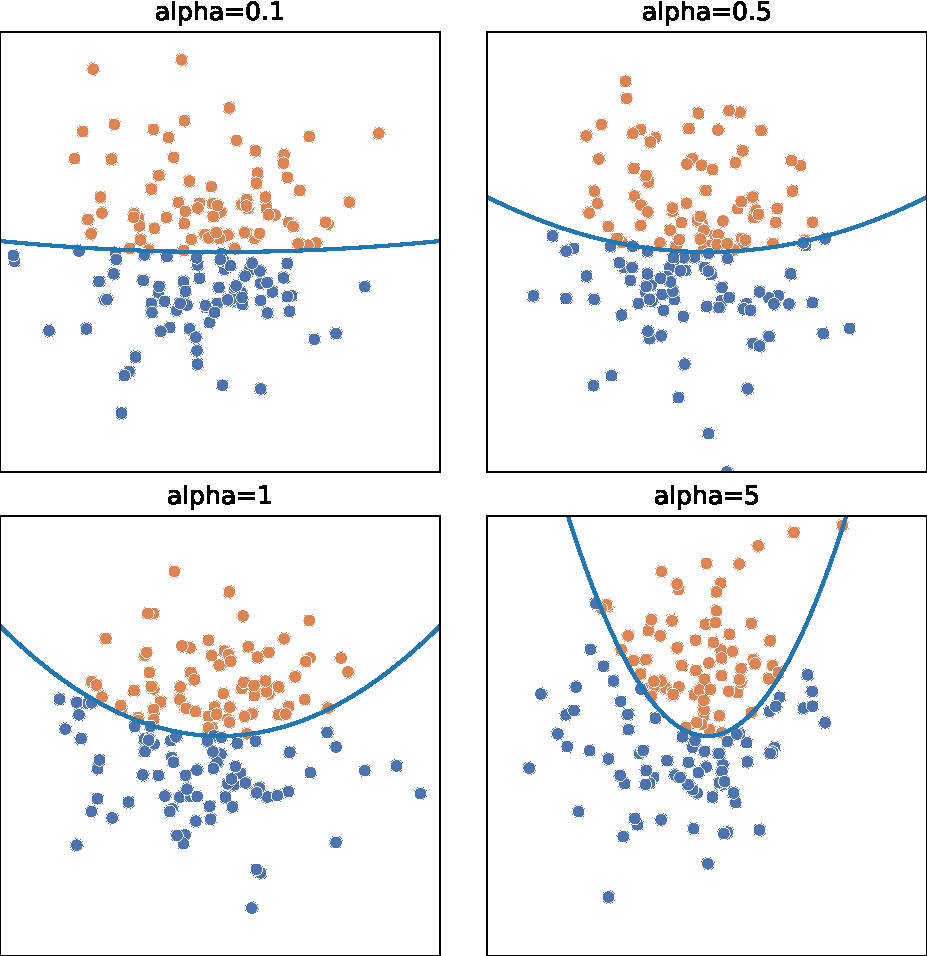
\includegraphics[width=.5\linewidth]{img/pacman_dataset_param_influence.pdf}
    \caption[Esempio di \emph{dataset} sintetici generati con funzione paraboloide.]{Esempio di \emph{dataset} sintetici generati con funzione paraboloide. Il parametro $\alpha$ controlla l'ampiezza.}
    \label{fig:pacman_dataset}
\end{figure}
A prescindere dalla funzione di etichettatura utilizzata, la procedura di generazione del \emph{dataset} è descritta nell'\Cref{alg:generazione_dataset_sintetici}.
Questa procedura richiede diversi parametri, descritti nell'elenco seguente.
\begin{itemize}
    \item Il parametro $n$ che identifica la dimensione totale del dataset.
    \item Il parametro \emph{seed} o seme, utilizzato per il generatore di numeri casuali.
    \item Il parametro \emph{test size} è la percentuale di $n$ da riservare come insieme di \emph{test}.
    \item Il parametro 
    \begin{equation*}
        p = \frac{\text{numero di elementi con etichetta positiva}}{\text{numero di elementi con etichetta negativa}}
    \end{equation*} 
    regola il bilanciamento tra le classi.
    \item Il parametro $r$ indica la percentuale di elementi della classe positiva e altrettanti esempi della classe negativa da selezionare a caso per poi invertirne l'etichetta.
\end{itemize}
\begin{algorithm}
    \SetAlgoLined
    \KwData{
        $n>0 \in \mathrm{N}$ dimensione del \emph{dataset} desiderata\\ 
        $p \in [0,1]$ per regolare il bilanciamento tra classi\\
        $r \in [0,1]$ per regolare la quantità di rumore\\
        \emph{test size} percentuale di dati da ritornare come \emph{test set}\\
        $s$ seme per le operazioni casuali\\
    }
    \KwResult{Dati $X$ ed etichette $y$ suddivisi in addestramento e test}
    Inizializza generatore casuale utilizzando il seme $s$\;
    $X_{\text{pop}} \gets$ seleziona a caso $10*n$ elementi\;
    $y_{\text{pop}} \gets$ etichetta $X_{\text{pop}}$ con la funzione di etichettatura\;
    %
    $N_p \gets \lfloor\frac{n}{p + 1}\rfloor$\;
    $N_n \gets n - N_p$\;
    $X, y \gets$ seleziona a caso $N_p$ elementi con etichetta positiva e $N_n$ elementi con etichetta negativa da $X_{\text{pop}},y_{\text{pop}}$\;
    seleziona a caso $\lfloor r * N_p \rfloor$\ esempi della classe positiva e $\lfloor r * N_n \rfloor$\ elementi della classe negativa a cui invertire l'etichetta\;
    $X_{\text{test}}, y_{\text{test}} \gets$ seleziona \emph{test size} elementi (con rispettive etichette) a caso come test set\;
    $X_{\text{train}} \gets X \setminus X_{\text{test}}$\;
    $y_{\text{train}} \gets y \setminus y_{\text{test}}$\;
\caption{Procedura generica per la generazione di \emph{dataset} sintetico.}
\label{alg:generazione_dataset_sintetici}
\end{algorithm}

% \subsubsection{Funzione sinusoidale}
% Fissando i parametri $\beta,\rho,\theta$, per un vettore $\Vec{x}=\{x_1,x_2\}$, l'etichetta $y$ è calcolata con la funzione
% \begin{equation}\label{eq:sinusoid_dataset_lf}
% lf(\Vec{x}) = \sign\left(\frac{1}{(1 + \exp(-\beta(x_1 - 0.5)) + \rho \sin(2\pi\theta x_1)} - x2\right).
% \end{equation}
% Questa funzione di etichettatura è utilizzata solo per dati in spazi con due dimensioni. La~\cref{fig:sinusoid_dataset} mostra alcuni esempi di \emph{dataset} e funzioni di etichettatura al variare dei parametri.
% \begin{figure}
%     \centering
%     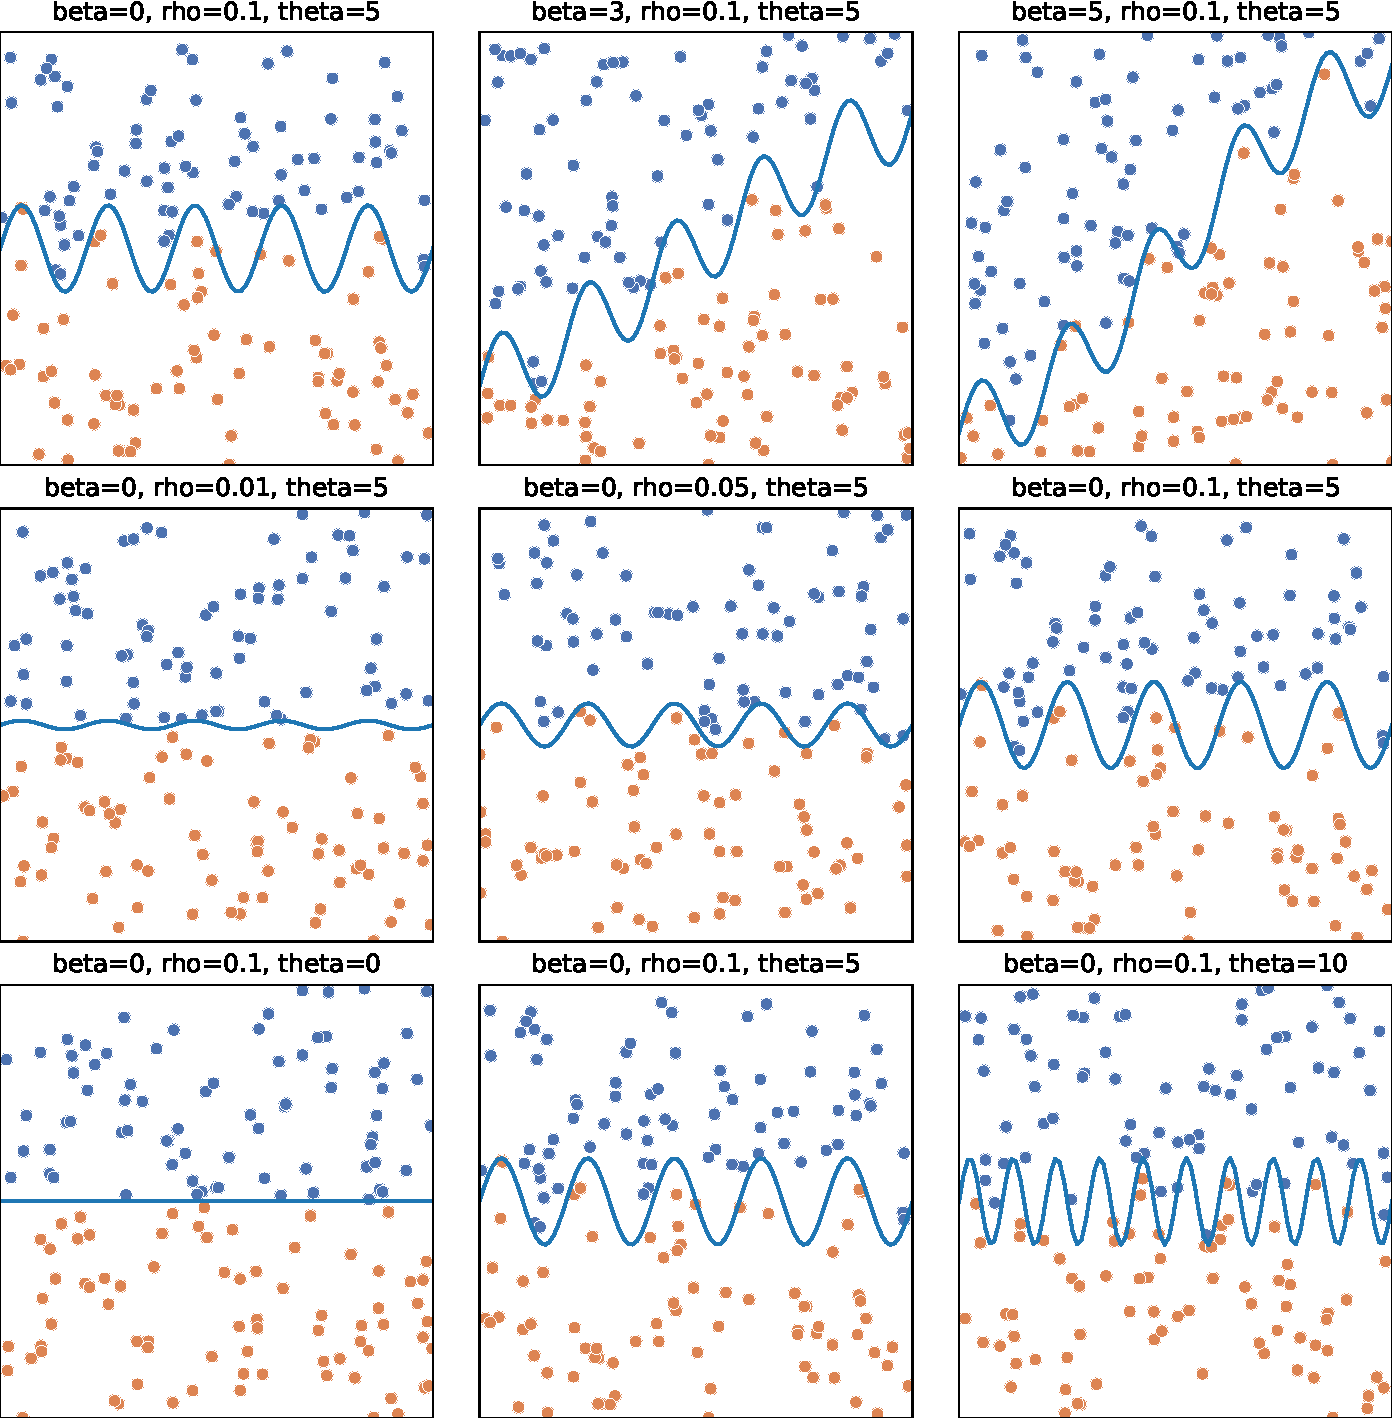
\includegraphics[width=1\linewidth]{img/sinusoid_dataset_param_influence.pdf}
%     \caption{Esempio di \emph{dataset} generati con funzione sinusoidale. 
%     $\beta$ controlla la pendenza, $\rho$ controlla l'ampiezza, $\theta$ la frequenza.}
%     \label{fig:sinusoid_dataset}
% \end{figure}
% \subsubsection{Funzione paraboloide}
% Fissati i parametri $\alpha, x_\text{shift}, y_\text{shift}$, per un vettore $\Vec{x}=\{x_1, \dots, x_n\} \in \mathrm{R}^n$, l'etichetta $y$ è calcolata con la funzione
% \begin{equation}\label{eq:pacman_dataset_lf}
% lf(\Vec{x})= x_n - \sum_{i=1}^{n-1}\alpha(x_i - x_\text{shift})^2 - y_\text{shift}.
% \end{equation}
% Il parametro $\alpha$ controlla l'ampiezza del paraboloide, mentre $x_\text{shift}$ e $y_\text{shift}$ traslano il vertice del paraboloide.
% La~\Cref{fig:pacman_dataset} mostra alcuni esempi di \emph{dataset} e funzioni di etichettatura al variare dei parametri.
% \begin{figure}
%     \centering
%     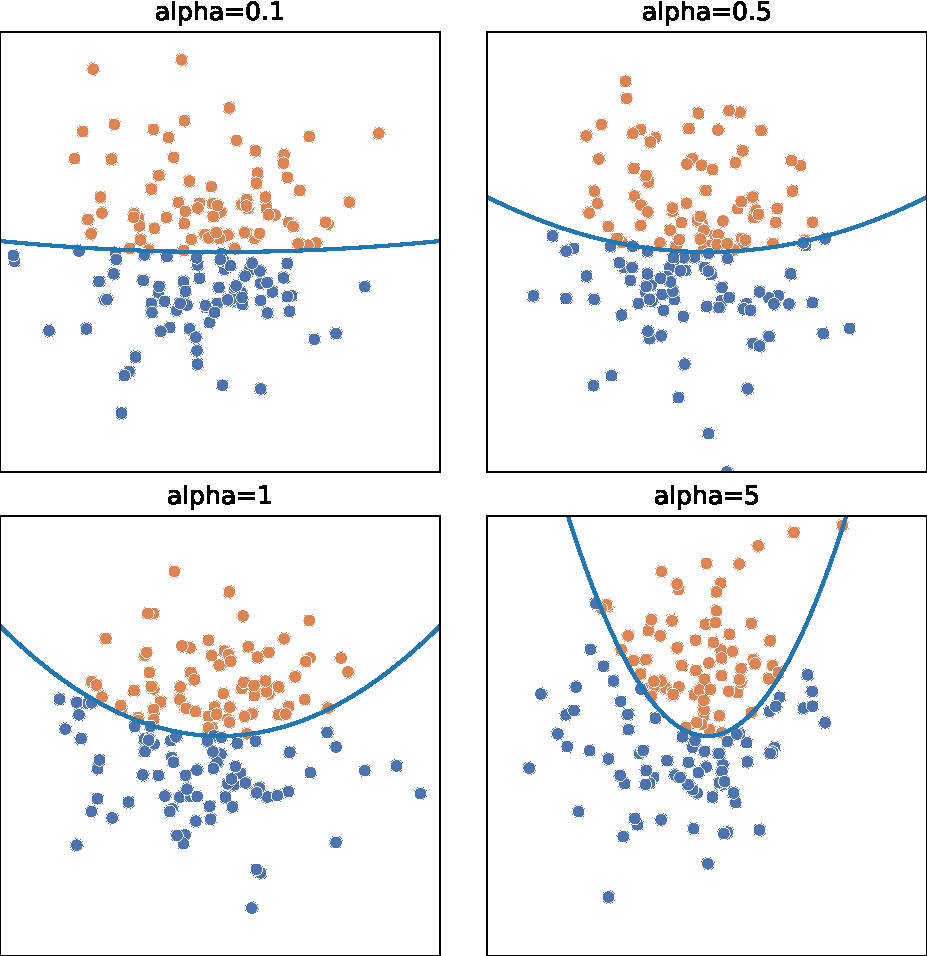
\includegraphics[width=1\linewidth]{img/pacman_dataset_param_influence.pdf}
%     \caption{Esempio di \emph{dataset} etichettati con paraboloide. Il parametro $\alpha$ controlla l'ampiezza.}
%     \label{fig:pacman_dataset}
% \end{figure}
I parametri per le funzioni di etichettatura utilizzati per la generazione dei \emph{dataset} sono scelti in modo da avere vari livelli di difficoltà di classificazione, misurata con le metriche esposte in~\Cref{sec:metriche_dataset}.
La difficoltà può essere gradualmente aumentata per esempio stringendo progressivamente il paraboloide o aumentando la frequenza o l'ampiezza della funzione sinusoidale.

La procedura nell'~\Cref{alg:generazione_dataset_sintetici} utilizza delle estrazioni casuali in diversi punti:
\begin{itemize}
    \item per selezionare la popolazione iniziale;
    \item per estrarre i dati di test;
    \item eventualmente nella procedura di introduzione del rumore, per selezionare degli esempi a cui invertire l'etichetta.
\end{itemize}

\subsection{Dataset di terze parti}
I \emph{dataset} di terze parti utilizzati per alcuni esperimenti provengono dalla pagina web della libreria LibSVM\footnote{\url{https://www.csie.ntu.edu.tw/~cjlin/libsvmtools/datasets/binary.html}}.
Sono \emph{dataset} utilizzati in letteratura ma pre-elaborati (scalando e normalizzando gli attributi) e resi disponibili in formato LibSVM~\cite{libsvm}.
Si riportano in~\Cref{tab:uci_datasets} le caratteristiche dei \emph{dataset} utilizzati.
\begin{table}
    \centering
    \begin{tabular}{cccc}
        \toprule
        Nome & Num. dati addestramento & Num. dati \emph{test} & Num. attributi\\
        \midrule
        svmguide1 &  3,089 & 4,000 & 4 \\
        a1a & 1,605	& 30,956 & 123\\
        gisette & 6000 & 1000 & 5000 \\
        \bottomrule
    \end{tabular}
    \caption{Caratteristiche \emph{dataset} di terze parti.}
    \label{tab:uci_datasets}
\end{table}


\section{Impostazione esperimenti}\label{sec:impostazione_esperimenti}
A prescindere dai \emph{dataset} utilizzati, la maggior parte degli esperimenti ha delle caratteristiche in comune:
\begin{itemize}
    \item la strategia utilizzata per definire le riduzioni di \emph{budget};
    \item il metodo di valutazione e selezione dei modelli;
    \item l'ambiente di esecuzione.
\end{itemize}
Questi aspetti sono discussi nei prossimi paragrafi.

\subsection{Strategia 1}
Il procedimento è descritto di seguito. Per prima cosa si addestra un modello SVM tradizionale senza nessun vincolo sul numero di vettori di supporto. Chiamiamo questo modello $FM$ e chiamiamo $FB$ il numero di vettori di supporto di $FM$.
In seguito, si addestrano una serie di modelli con un \emph{budget} pari a una frazione di $FB$.
Per ognuno di questi modelli il \emph{budget} è espresso come $B=p*FM$, dove
\begin{equation*}
    p\in\{0.3, 0.4, 0.5, 0.6, 0.7, 0.8, 0.9\}.
\end{equation*}
Nei grafici dei risultati ottenuti con questa strategia compare anche il valore di \emph{budget} $p=1$: indica dei modelli classici senza nessun vincolo di \emph{budget}.
Nell'~\Cref{alg:esperimenti_1} è descritto lo pseudocodice per la strategia.
\begin{algorithm}
    \SetAlgoLined
    \KwData{\emph{dataset} da analizzare}
    %\KwResult{}
    $FM \gets$ seleziona il miglior modello senza imporre nessun vincolo di \emph{budget}\;
    $FB \gets$ numero di vettori di supporto del modello $FM$\;
    salva parametri e dettagli di $FM$\;
    \For{$p\gets0.3$ \KwTo $0.9$ \KwBy $0.1$}{
        $B\gets p*FB$\;
        $M \gets$ seleziona il miglior modello con $\text{budget}=B$\;
        salva parametri e dettagli di $M$\;
    }
\caption{Pseudocodice strategia 1.}
\label{alg:esperimenti_1}
\end{algorithm}

Utilizzando questa strategia è possibile misurare l'accuratezza sui dati di \emph{test} al diminuire del \emph{budget} e paragonarla all'accuratezza del corrispettivo modello classico addestrato sullo stesso dataset.
Per ogni modello, si definisce \emph{score ratio} la quantità
\begin{equation*}
    \text{score ratio} = \frac{\text{accuratezza su dati di \emph{test} del modello \emph{budgeted SVC}}}{\text{accuratezza su dati di \emph{test} del corrispettivo modello classico}}.
\end{equation*}

Con questi esperimenti è possibile ottenere delle indicazioni su quanto sia possibile ridurre il \emph{budget} senza penalizzare troppo l'accuratezza, limitatamente ai \emph{dataset} considerati e in rapporto alla controparte senza vincolo sul \emph{budget}.

Per mitigare un eventuale \emph{bias} dovuto alla casualità nella generazione del dataset, si è deciso in alcuni casi di generare tre \emph{dataset} per ogni gruppo di parametri utilizzando altrettanti valori del parametro seme.
La procedura completa, in questo caso, è descritta nell'~\Cref{alg:esperimenti_2}.
\begin{algorithm}
    \SetAlgoLined
    \KwData{parametri \emph{dataset} $\gets$ le varie combinazioni di parametri per generare dataset.}    
    \For{$s \gets \text{estrai nuovo seme}$}{
        \For{params \KwIn \text{parametri dataset}}{
            $ds\gets$ genera \emph{dataset} con l'~\Cref{alg:generazione_dataset_sintetici} usando $params$ e $s$\;
            esegui l'~\Cref{alg:esperimenti_1} su $ds$\;           
        }
    }
\caption{Pseudocodice esperimenti con strategia 1 e con ripetizione della generazione dei dataset.}
\label{alg:esperimenti_2}
\end{algorithm}

\subsection{Strategia 2}
Un secondo approccio per eseguire gli esperimenti su un certo \emph{dataset} consiste nell'esprimere il \emph{budget} in funzione alla dimensione del \emph{dataset} invece che in funzione al numero di vettori di supporto di un modello classico.
Questa strategia è descritta nell'~\Cref{alg:esperimenti_3}.
\begin{algorithm}
    \SetAlgoLined
    \KwData{\emph{dataset}}
    %\KwResult{}
    $m \gets |\textit{dataset}|$\;
    \For{$p$ \KwIn $\{0.01, 0.025, 0.05, 0.075, 0.1, 0.125, 0.15, 0.175, 0.2\}$}{
        $B\gets pm$\;
        $M \gets$ seleziona il miglior modello con \emph{budget} $B$ su \emph{dataset}\;
        salva parametri e dettagli di $M$\;
    }
\caption{Pseudocodice strategia 2.}
\label{alg:esperimenti_3}
\end{algorithm}
Per un certo \emph{dataset} composto da $m$ elementi, si esprime il \emph{budget} come $B=pm$, dove
\begin{equation*}
    p\in\{0.01, 0.025, 0.05, 0.075, 0.1, 0.125, 0.15, 0.175, 0.2\}.
\end{equation*}
Così facendo è possibile verificare la bontà dei modelli con un \emph{budget} molto stringente, fino all'$1\%$ dei dati di addestramento.

Per gli esperimenti effettuati con questa strategia, i \emph{dataset} sintetici sono stati generati una sola volta con un solo seme per ogni configurazione di parametri.

\subsection{Selezione e valutazione modelli}
Ogni modello è valutato sullo stesso insieme di dati di \emph{test} per ogni \emph{dataset}.
Nel caso dei dati di terze parti, l'insieme di \emph{test} è già fornito, mentre nel caso di dati sintetici l'insieme di \emph{test} viene selezionato dopo la procedura di generazione e non viene più modificato.
L'insieme di \emph{test} è scelto casualmente, ma mantiene il bilanciamento delle classi dei dati di addestramento.

I migliori iperparametri sono selezionati sui dati di addestramento utilizzando \emph{5-fold cross validation}, con una ricerca esaustiva sulla griglia di parametri descritta in~\Cref{tab:gridsearch_2d}.
\begin{table}
    \centering
    \begin{tabular}{cccc}
        \toprule
        $C$ & \emph{Kernel} & $\gamma$ & d \\
        \midrule
        \multirow{3}{*}{[0.01, 0.1, 1, 10]} & Gaussiano   & [0.0001, 0.001, 0.01, 0.1, 1, 10]   & /\\
                                            \cline{2-4}
                                            & Polinomiale   & / & [2, 5, 10] \\
                                            \cline{2-4}
                                            & Lineare       & / & / \\
        \bottomrule
    \end{tabular}
    \caption{Griglia di iperparametri per selezionare i modelli \emph{budgeted SVC}.}
    \label{tab:gridsearch_2d}
\end{table}
Questi parametri sono riferiti al metodo \emph{budgeted SVC}; nel caso in cui un esperimento sia stato eseguito con una griglia differente, sarà specificato nel paragrafo che lo descrive.

\subsection{Ambiente di esecuzione}
Tutti gli esperimenti sono stati eseguiti su un server con CPU Intel(R) Xeon(R) W-1250P CPU @ 4.10GHz e con 31GB di ram. Il linguaggio di programmazione utilizzato è Python 3.10.10. \`E stato utilizzato il risolutore Gurobi 10.0.1~\cite{gurobi}. 

Per cercare di ridurre il carico computazionale, gli esperimenti effettuati utilizzando la formulazione \emph{budgeted SVC} utilizzano una matrice \emph{kernel} pre-calcolata; le implementazioni di altri metodi presenti in letteratura utilizzati come confronto, invece, calcolano i valori di \emph{kernel} durante l'addestramento.

Il limite massimo di tempo concesso al risolutore per risolvere ogni istanza è di sessanta secondi.

\section{Esperimenti su dataset sintetici 2D}\label{sec:exp:synth_2d}
Si riportano in questo paragrafo gli esperimenti effettuati sui \emph{dataset} sintetici generati con le configurazioni di parametri riportate nelle~\Cref{tab:parametri_ds_sin,tab:parametri_ds_pacman}.
\begin{table}
    \centering
    \begin{tabular}{ccccc}
        \toprule
         $n$ & \emph{test size} & $\beta$ & $\rho$ & $\theta$ \\
        \midrule
        \multirow{10}{*}{1000} & \multirow{10}{*}{0.3} &\multirow{5}{*}{0}  & 0.01  & \multirow{5}{*}{20} \\        
                            &&& 0.025 &     \\        
                            &&& 0.05  &     \\        
                            &&& 0.075 &     \\        
                            &&& 0.1   &     \\
        \cline{3-5}
                &&  95      & 0.2   & 10    \\   
        \cline{3-5}
        &&  \multirow{4}{*}{0}  & \multirow{4}{*}{0.1}  & 1     \\    
                            &&&                       & 2     \\    
                            &&&                       & 5     \\    
                            &&&                       & 1     \\    
        \bottomrule
    \end{tabular}
    \caption{Configurazioni di parametri utilizzati per generare \emph{dataset} bidimensionali con la funzione sinusoidale in~\Cref{eq:sinusoid_dataset_lf}.}
    \label{tab:parametri_ds_sin}
\end{table}
\begin{table}
    \centering
    \begin{tabular}{ccccc}
        \toprule
         $n$ & \emph{test size} &$\alpha$ & $x_\text{shift}$ & $y_\text{shift}$ \\
        \midrule
        \multirow{5}{*}{1000} & \multirow{5}{*}{0.3} &1   & \multirow{5}{*}{0.5} & \multirow{5}{*}{0.5} \\
        && 2.5 &\\
        && 5   &\\
        && 7.5 &\\
        && 10  &\\
        \bottomrule
    \end{tabular}
    \caption{Configurazioni di parametri utilizzati per generare \emph{dataset} bidimensionali con la funzione paraboloide in~\Cref{eq:pacman_dataset_lf}.}
    \label{tab:parametri_ds_pacman}
\end{table}

\subsubsection{Esperimenti utilizzando la strategia 1}
In~\Cref{fig:risultati_2d} si riportano dei grafici che riportano l'andamento dell'accuratezza e dello \emph{score ratio} ottenuti sui dati di \emph{test} al variare del \emph{budget}.
Questa figura mostra solo i risultati più significativi; i grafici omessi sono riportati nell'Appendice A.

Dai risultati ottenuti è possibile notare come per \emph{dataset} semplici, o con una funzione di etichettatura sinusoidale con tante oscillazioni ma ben approssimabile da una superficie lineare, il metodo proposto risulta efficace, portando a una riduzione significativa del numero di vettori di supporto senza pagare troppo in termini di accuratezza.
In altri casi, invece, con \emph{dataset} più difficili, il comportamento è diverso:
\begin{itemize}
    \item per piccole riduzioni di \emph{budget}, come $80\%$ e $90\%$ del numero di vettori di supporto del modello tradizionale, la perdita in accuratezza è moderata;
    \item per valori di \emph{budget} intermedi nel range considerato, tra il $40\%$ e il $70\%$ la perdita di accuratezza è più grave e marcata;
    \item per valori di \emph{budget} piccoli, come $30\%$ o $40\%$, l'accuratezza è migliore di quella ottenuta per diminuzioni di \emph{budget} tra il $40\%$ e il $70\%$.
\end{itemize}
Sempre per i \emph{dataset} più difficili, si nota anche un'alta variabilità nei risultati ottenuti nel gruppo di \emph{dataset} generati con stessi parametri ma seme diverso, con alcune istanze che esibiscono accuratezza molto bassa.
Dalla~\Cref{fig:risultati_2d} è possibile notare come i modelli peggiori siano associati a un'istanza del problema \emph{budgeted SVC} non risolta all'ottimo, perché il risolutore ha raggiunto il limite massimo di tempo concesso e ha restituito una soluzione non ottimale.
L'interpretazione è quindi che per riduzioni di \emph{budget} intermedie, il risolutore faccia più fatica a modellare la funzione originale perché non può utilizzare abbastanza vettori di supporto, mentre invece per \emph{budget} più ristretti la soluzione del problema sia più semplice perché è possibile escludere più velocemente un maggior numero di soluzioni.

Nei casi in cui si riscontra alta variabilità (utilizzando la stesa riduzione di \emph{budget} sullo stesso gruppo di \emph{dataset}) si può notare come si ottengano anche modelli buoni, spesso costruiti con una soluzione ottima.
\begin{figure}
    \begin{subfigure}{.5\textwidth}
        \centering
        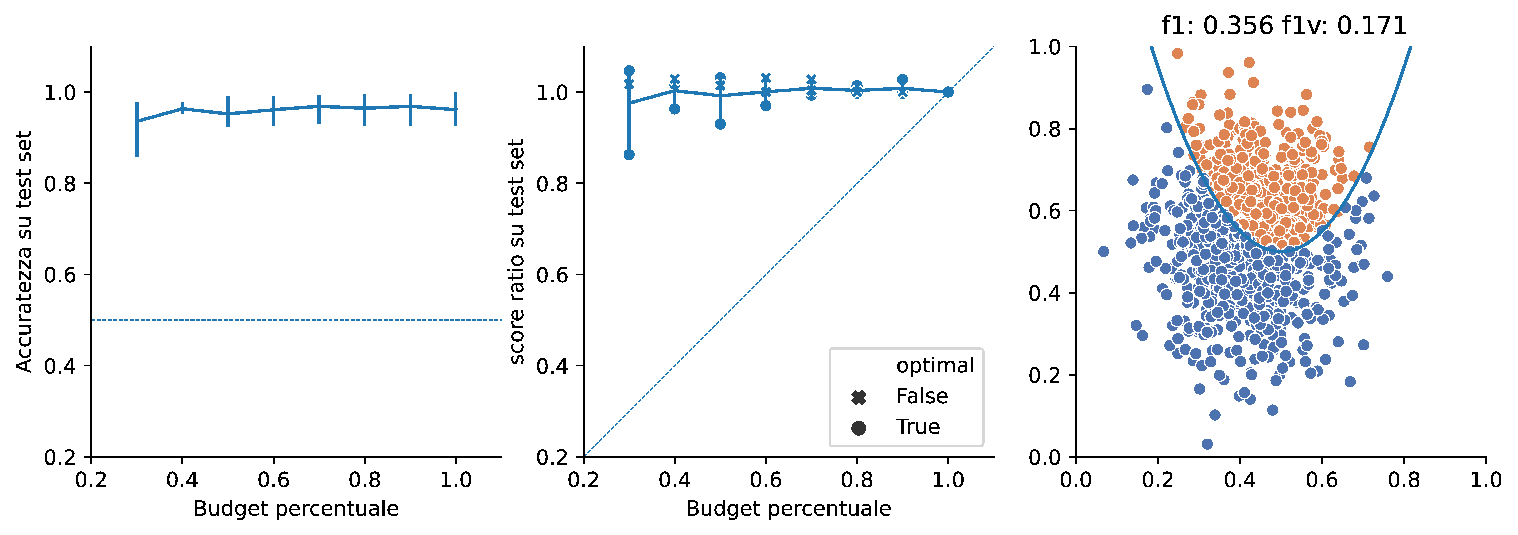
\includegraphics[width=\textwidth]{img/2d/3.pdf}
    \end{subfigure}%
    \begin{subfigure}{.5\textwidth}
        \centering
        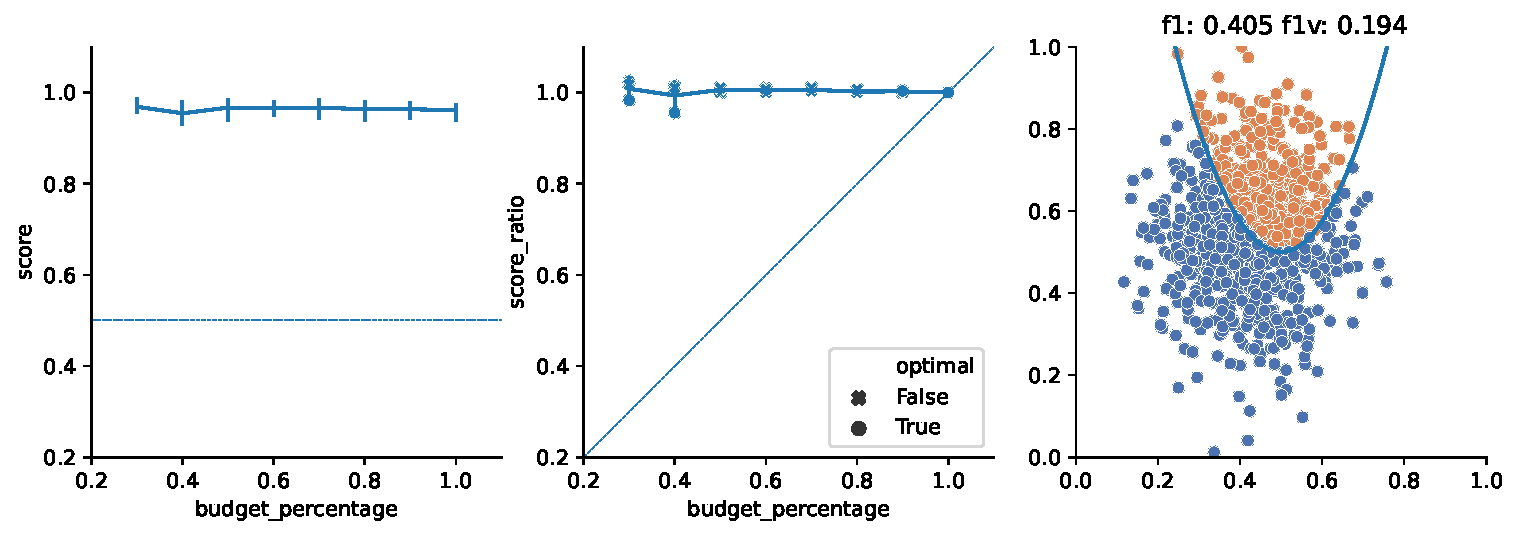
\includegraphics[width=\textwidth]{img/2d/4.pdf}
    \end{subfigure}%
    %
    \hfill
    %
    \begin{subfigure}{.5\textwidth}
        \centering
        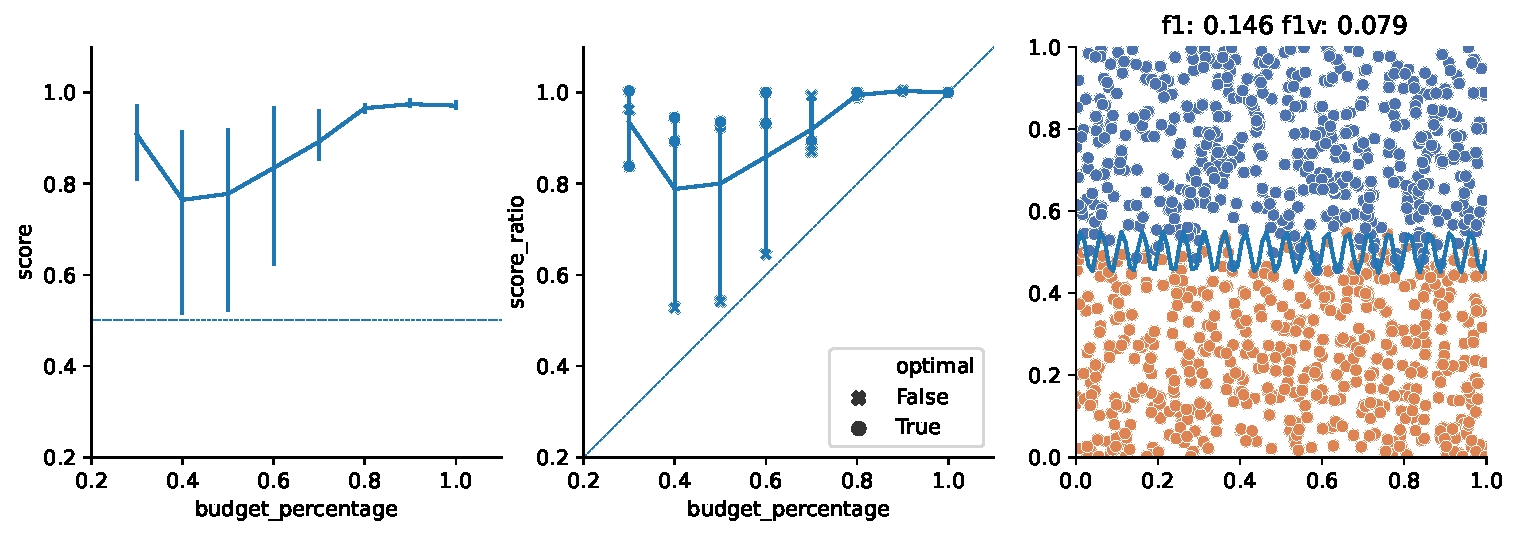
\includegraphics[width=\textwidth]{img/2d/8.pdf}
    \end{subfigure}%
    \begin{subfigure}{.5\textwidth}
        \centering
        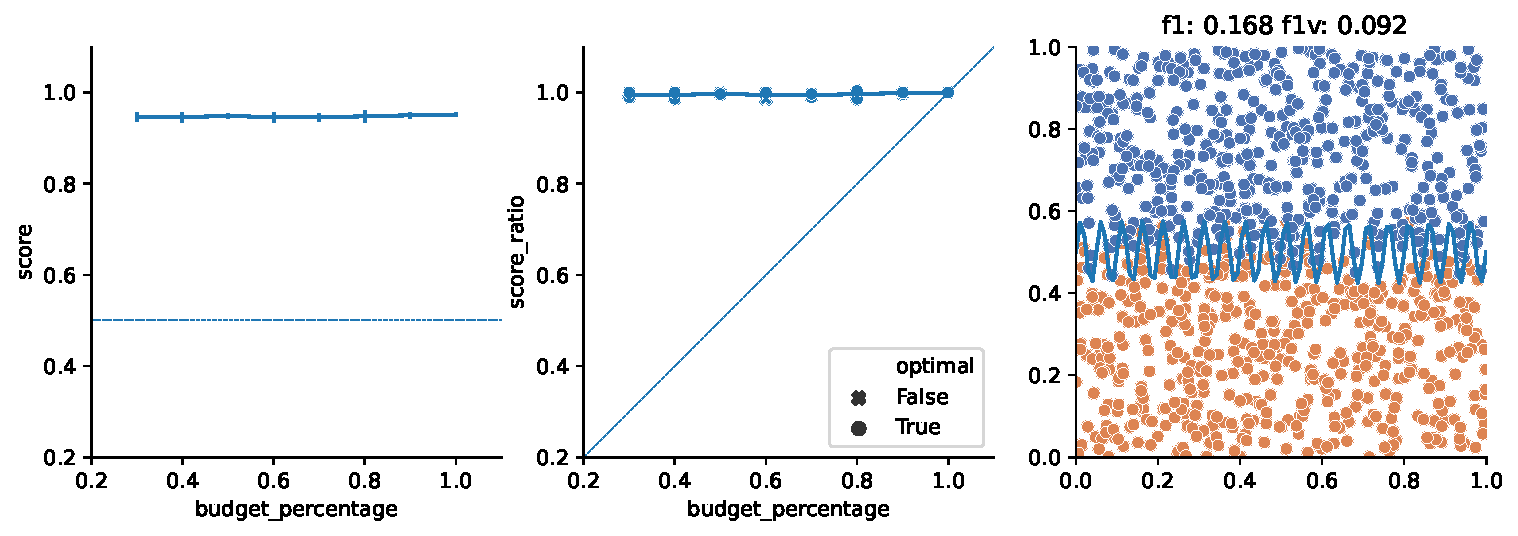
\includegraphics[width=\textwidth]{img/2d/9.pdf}
    \end{subfigure}%
    %
    \hfill
    %
    \begin{subfigure}{.5\textwidth}
        \centering
        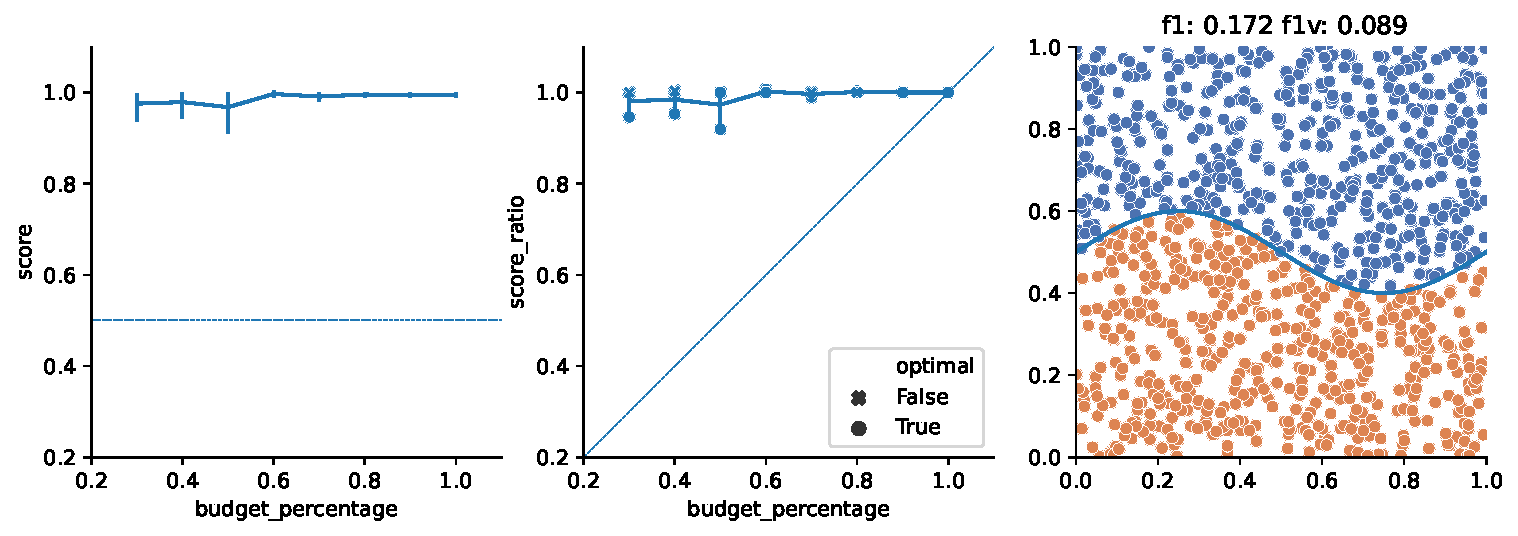
\includegraphics[width=\textwidth]{img/2d/10.pdf}
    \end{subfigure}%
    \begin{subfigure}{.5\textwidth}
        \centering
        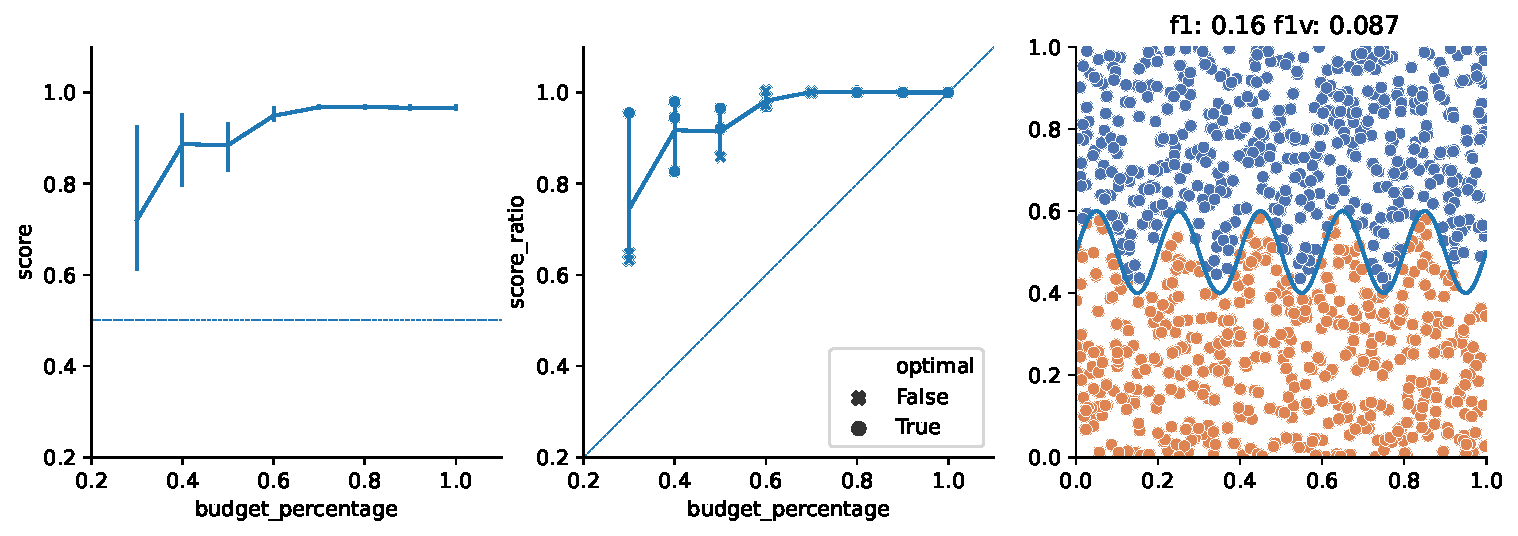
\includegraphics[width=\textwidth]{img/2d/12.pdf}
    \end{subfigure}%
     %
    \hfill
    %
    \begin{subfigure}{.5\textwidth}
        \centering
        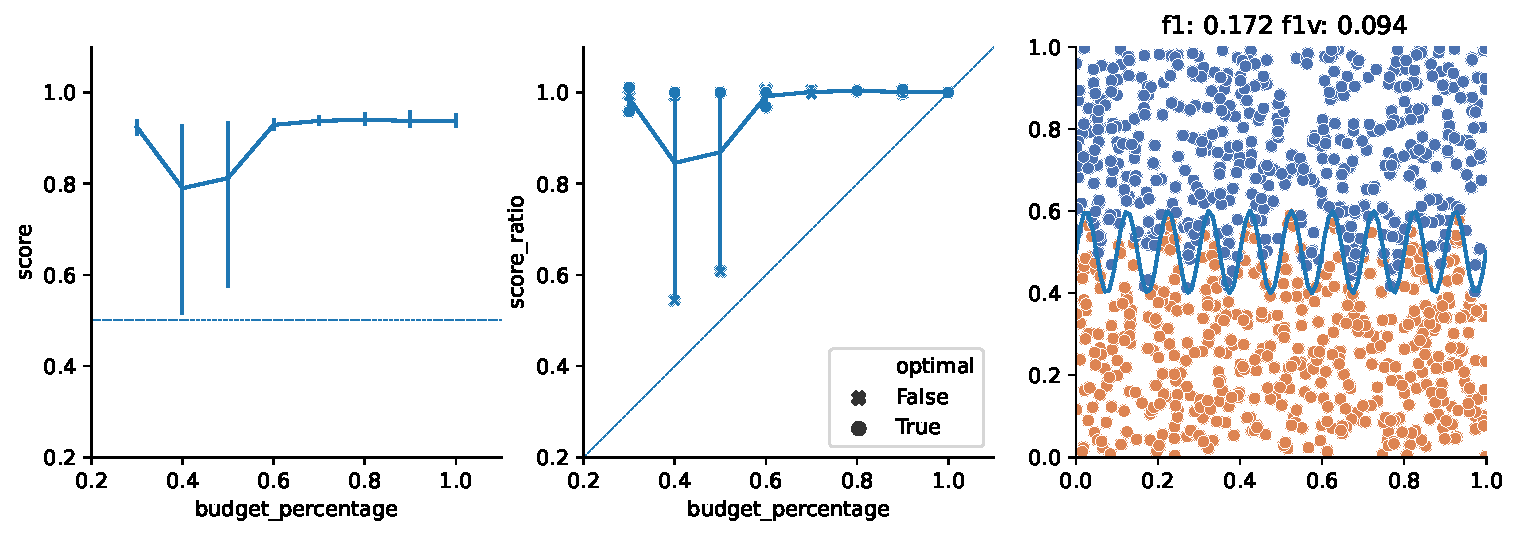
\includegraphics[width=\textwidth]{img/2d/13.pdf}
    \end{subfigure}%
    \begin{subfigure}{.5\textwidth}
        \centering
        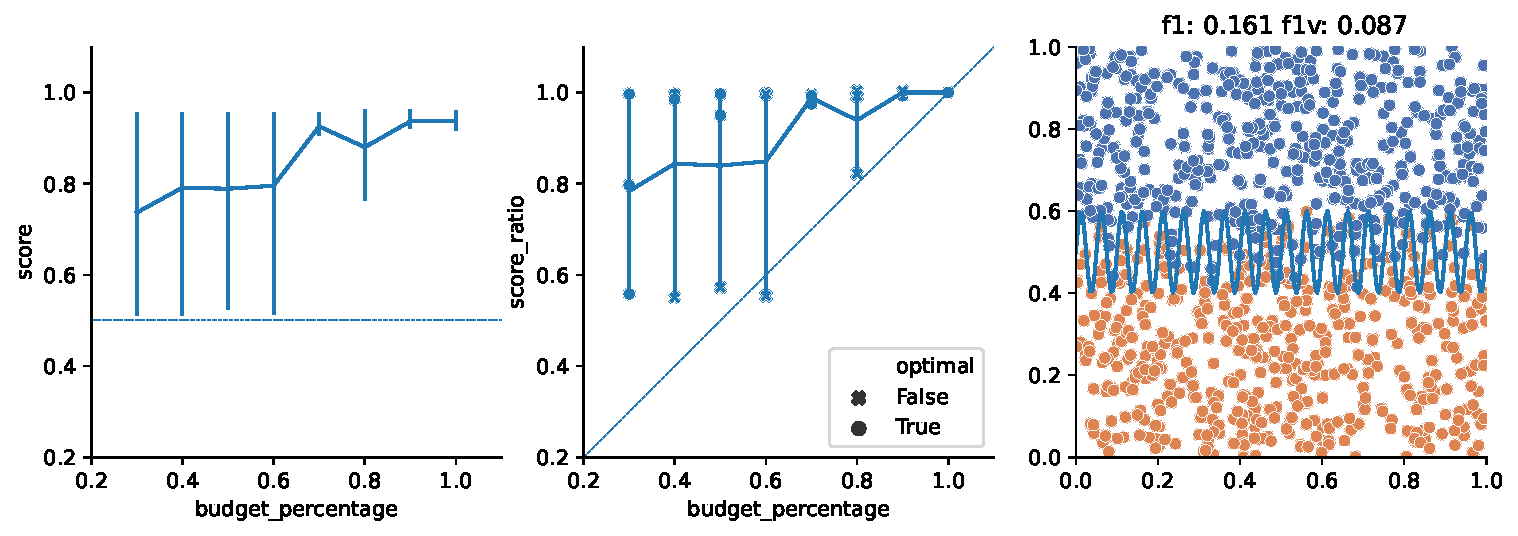
\includegraphics[width=\textwidth]{img/2d/14.pdf}
    \end{subfigure}%
     %
    \hfill
    %
    \begin{subfigure}{.5\textwidth}
        \centering
        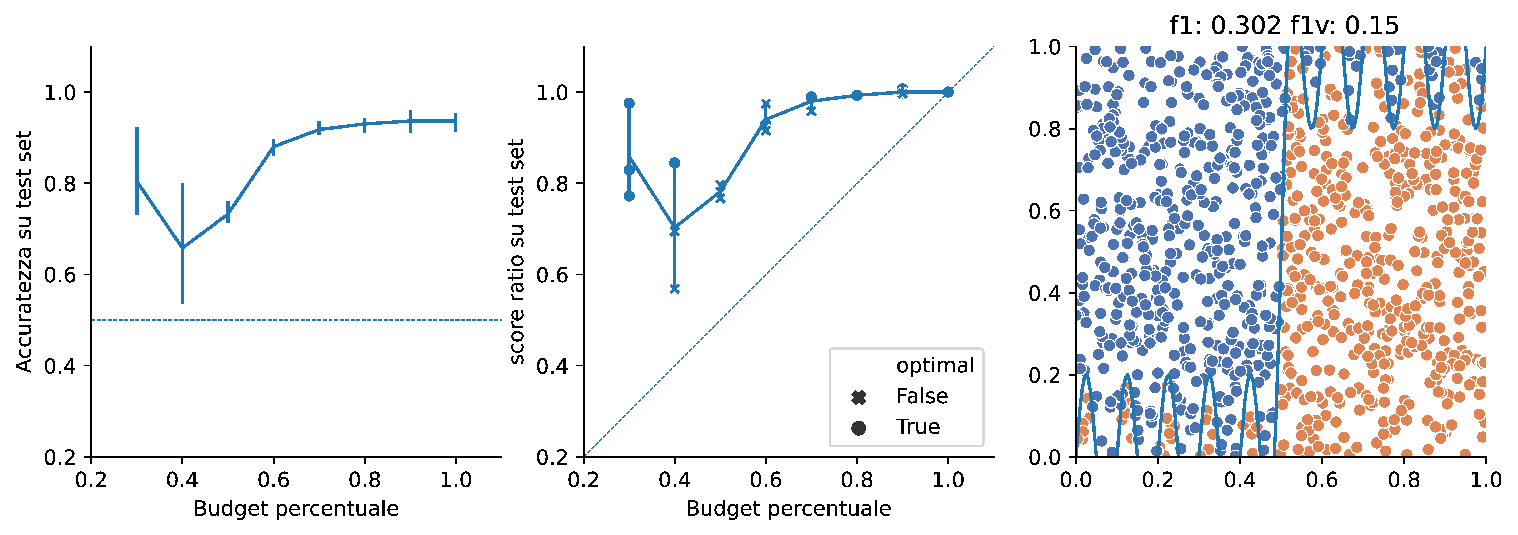
\includegraphics[width=\textwidth]{img/2d/15.pdf}
    \end{subfigure}%
    \caption[Risultati su \emph{dataset} sintetici utilizzando la strategia 1.]{Risultati più significativi ottenuti su \emph{dataset} sintetici 2D utilizzando la strategia 1. Ognuno dei grafici a sinistra indica l'andamento dell'accuratezza sui dati di \emph{test} al variare del \emph{budget}; ognuno dei grafici al centro indica lo \emph{score ratio} al variare del \emph{budget} (un simbolo ``x'' indica che il risolutore ha ritornato una soluzione non ottima); ognuno dei grafici a destra rappresenta uno dei tre \emph{dataset} utilizzati con le rispettive metriche di difficoltà.}
\label{fig:risultati_2d}
\end{figure}

% magari full_budget partiva già con "pochi" sv e ridurli porta ad accuracy molto più basse... ma non so

Analizzando il numero di vettori di supporto dei modelli tradizionali,~\Cref{fig:2d_dist_numsv}, è possibile notare come la maggior parte dei modelli abbia un numero ragionevole di vettori di supporto ma come una minoranza abbia invece un numero molto elevato.
\begin{figure}
    \centering
    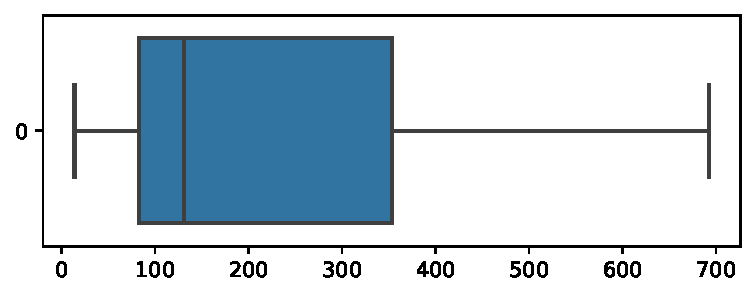
\includegraphics[width=0.5\linewidth]{img/2d/numsv.pdf}
    \caption{Distribuzione del numero di vettori di supporto per i modelli classici addestrati sui \emph{dataset} sintetici con la strategia 1.}
    \label{fig:2d_dist_numsv}
\end{figure}

\subsubsection{Risultati ottenuti utilizzando la strategia 2}
Utilizzando gli stessi \emph{dataset} dell'esperimento precedente, sono stati effettuati ulteriori esperimenti utilizzando la strategia 2.
In~\Cref{fig:2d_v2} si riporta l'andamento dell'accuratezza sui dati di \emph{test} al variare del \emph{budget} per ogni \emph{dataset}.
Questa figura mostra solo i risultati più significativi; i grafici omessi sono riportati nell'Appendice A.

\begin{figure}
    \begin{subfigure}{.5\textwidth}
        \centering
        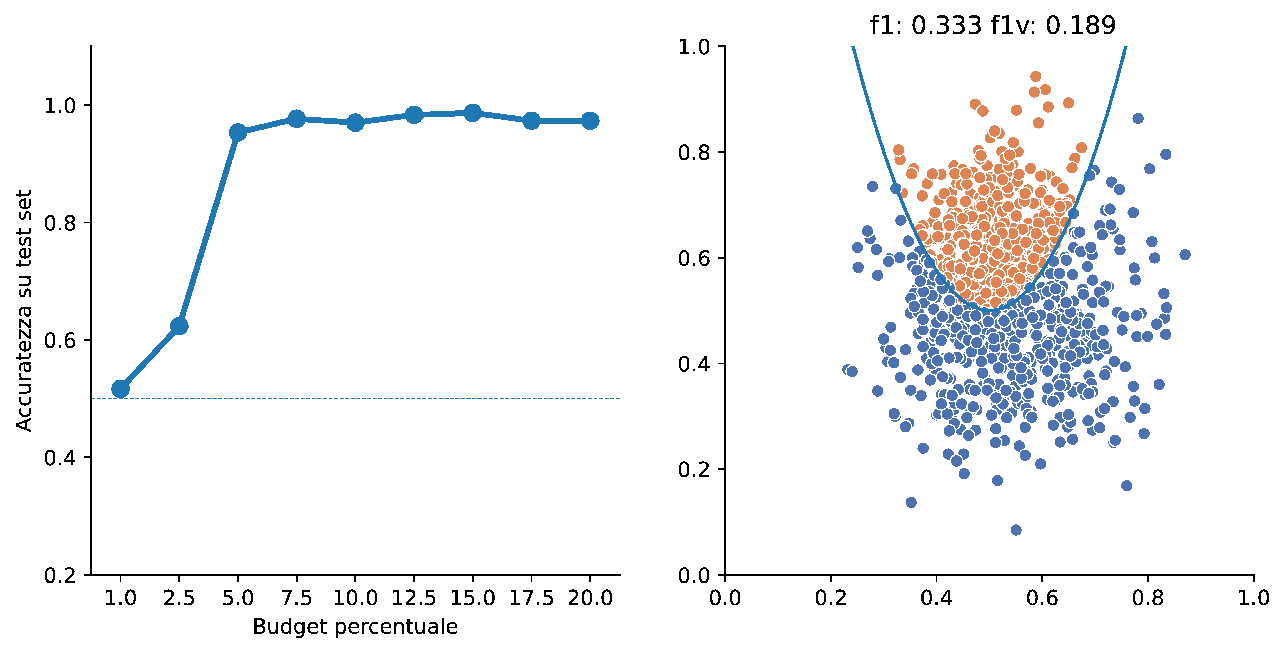
\includegraphics[width=\textwidth]{img/2d_v2/4.pdf}
    \end{subfigure}%
    \begin{subfigure}{.5\textwidth}
        \centering
        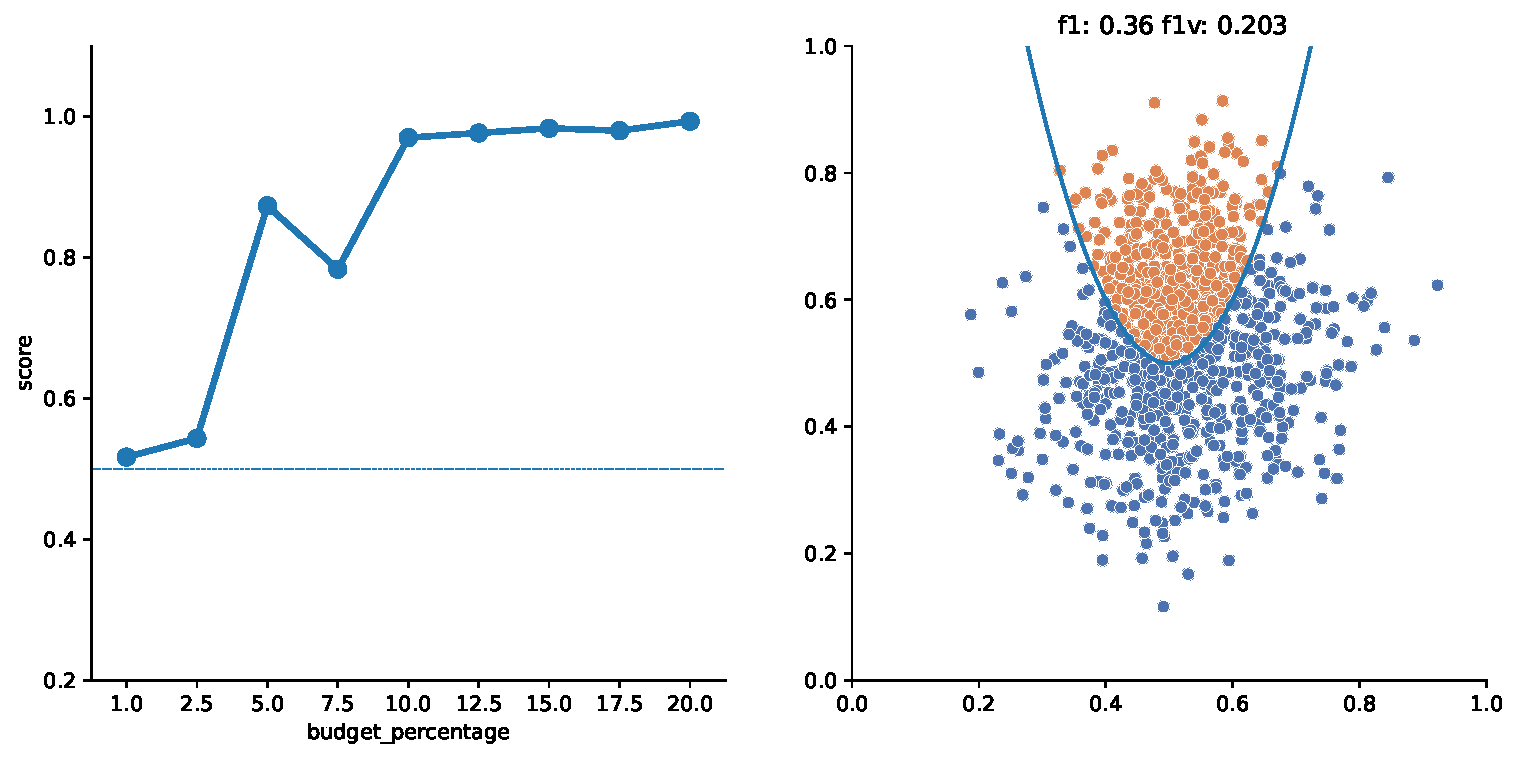
\includegraphics[width=\textwidth]{img/2d_v2/5.pdf}
    \end{subfigure}
    %
    \hfill
    %
    \begin{subfigure}{.5\textwidth}
        \centering
        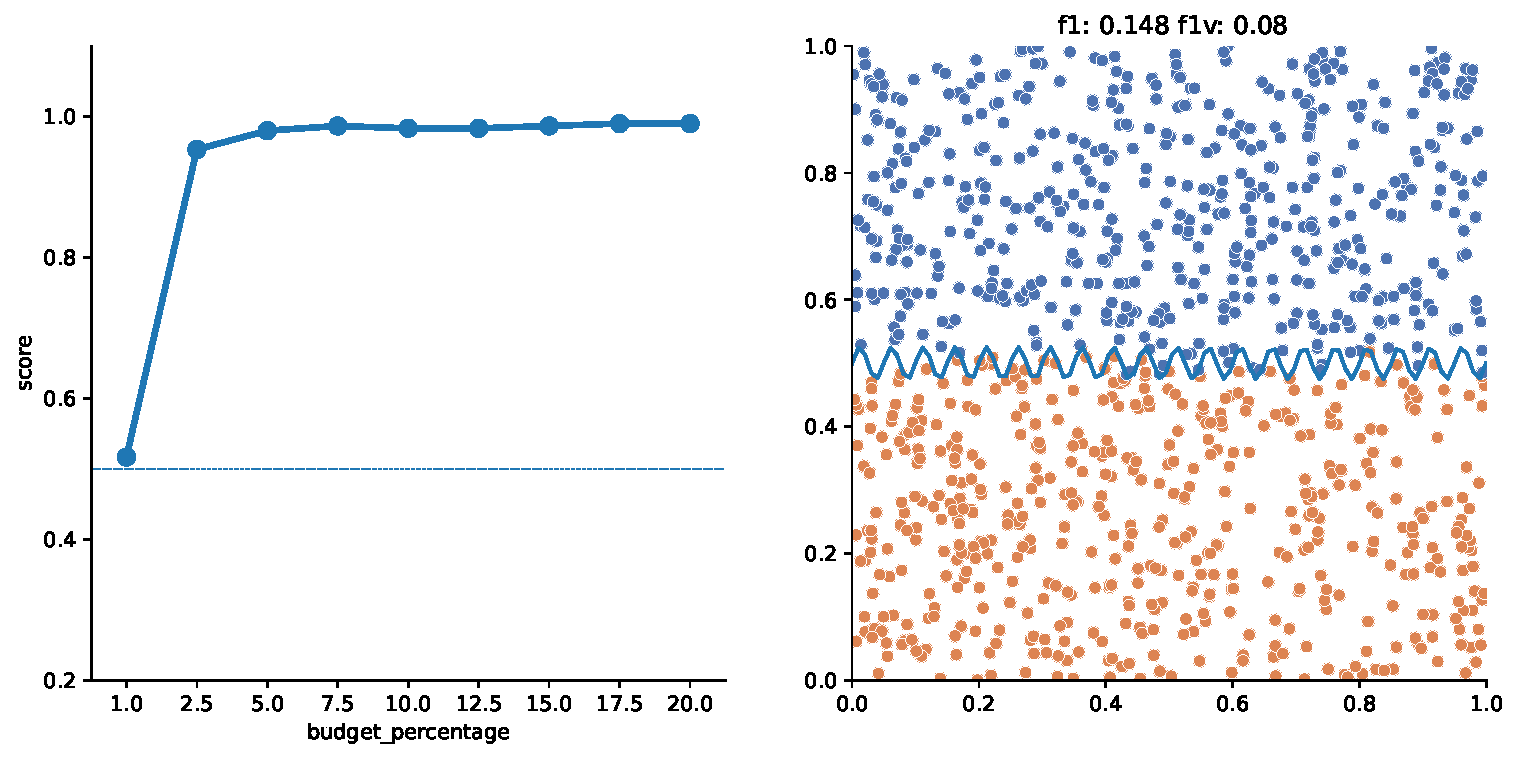
\includegraphics[width=\textwidth]{img/2d_v2/7.pdf}
    \end{subfigure}
    \begin{subfigure}{.5\textwidth}
        \centering
        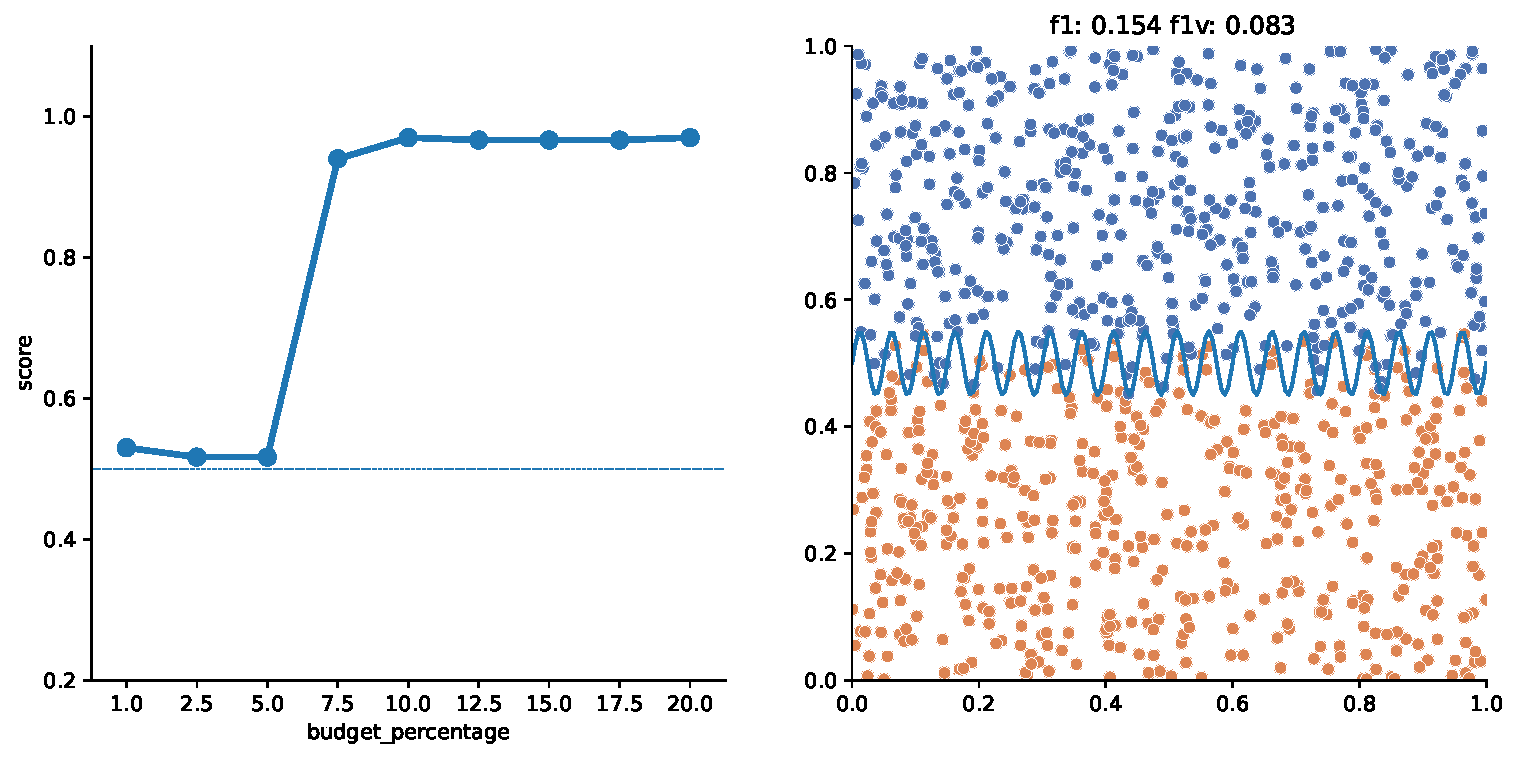
\includegraphics[width=\textwidth]{img/2d_v2/8.pdf}
    \end{subfigure}%
    %
    \hfill
    %
    \begin{subfigure}{.5\textwidth}
        \centering
        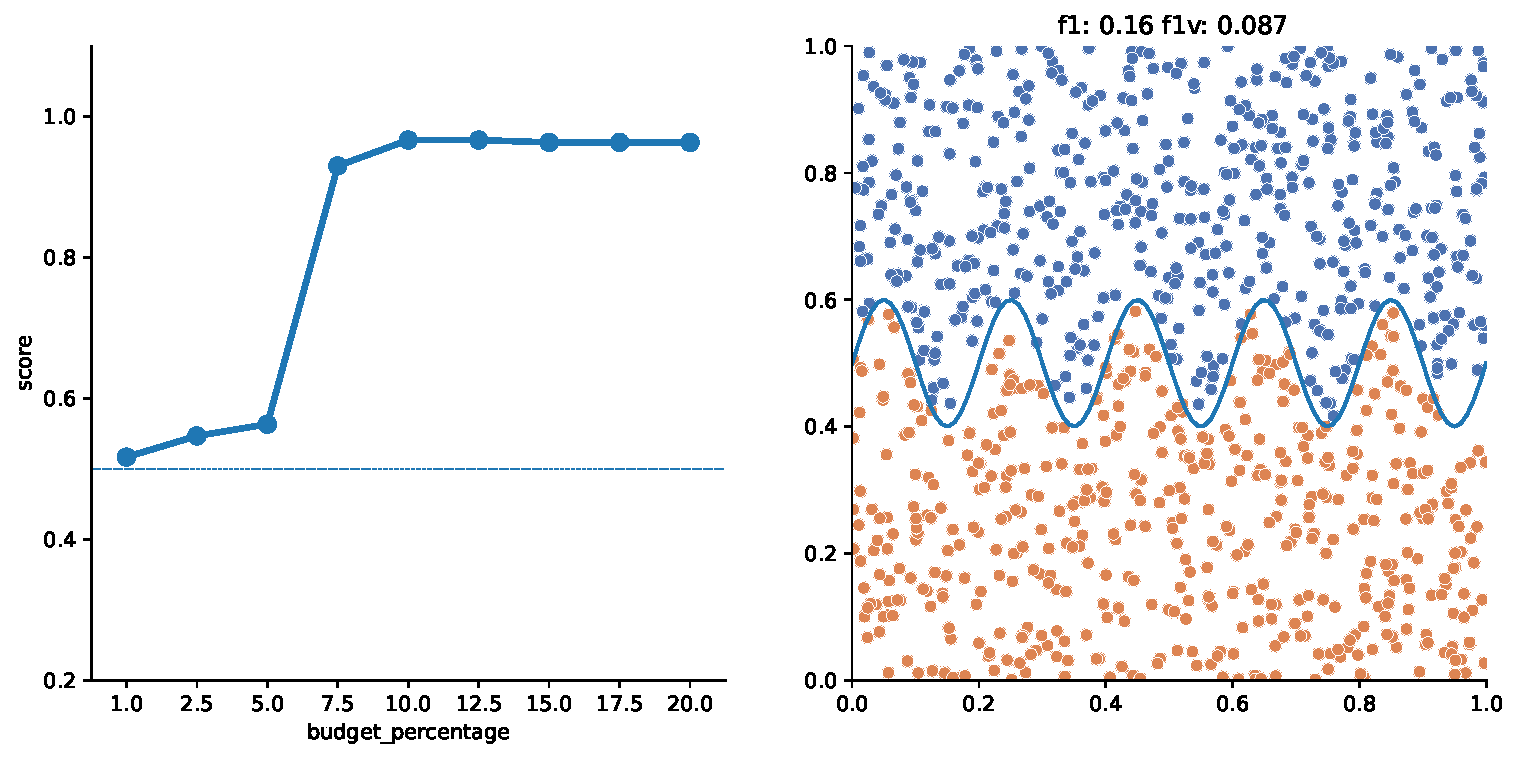
\includegraphics[width=\textwidth]{img/2d_v2/12.pdf}
    \end{subfigure}
    \begin{subfigure}{.5\textwidth}
        \centering
        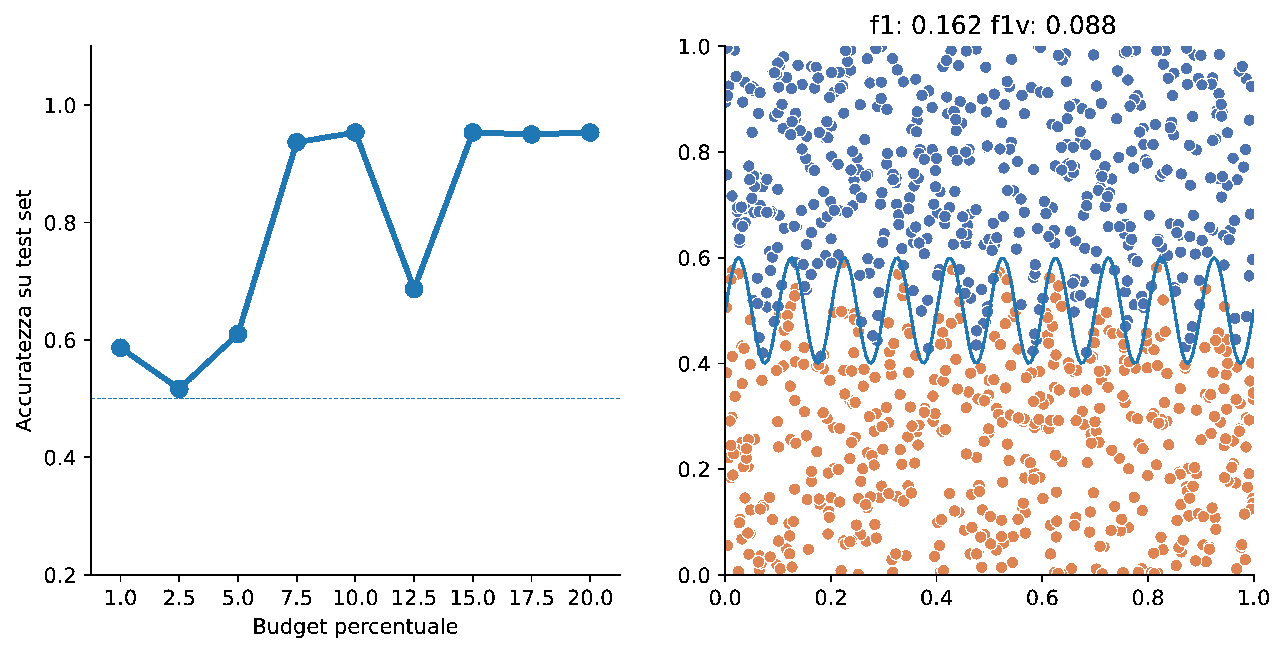
\includegraphics[width=\textwidth]{img/2d_v2/13.pdf}
    \end{subfigure}%
    %
    \hfill
    %
    \begin{subfigure}{.5\textwidth}
        \centering
        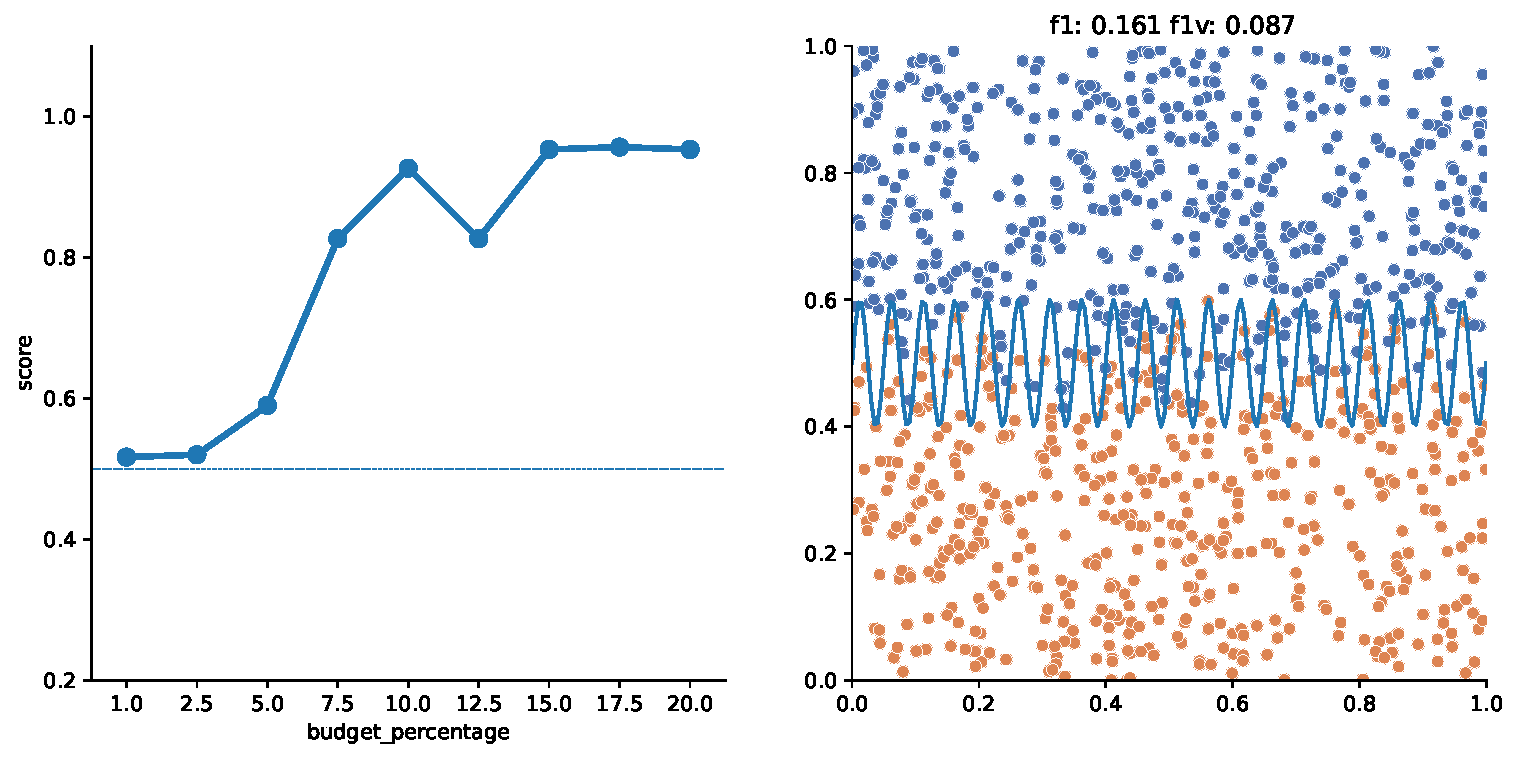
\includegraphics[width=\textwidth]{img/2d_v2/14.pdf}
    \end{subfigure}
    \begin{subfigure}{.5\textwidth}
        \centering
        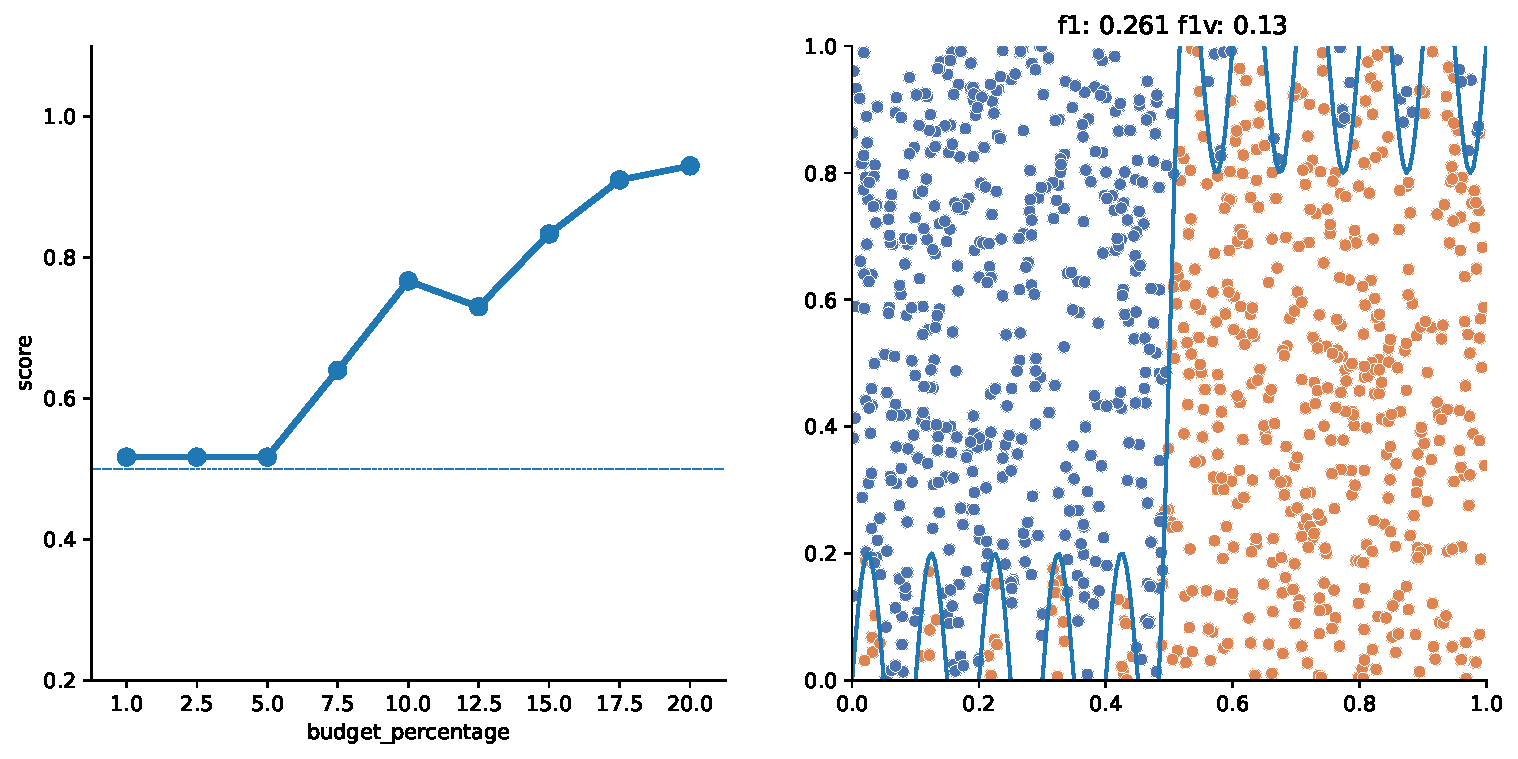
\includegraphics[width=\textwidth]{img/2d_v2/15.pdf}
    \end{subfigure}%
\caption[Risultati su \emph{dataset} sintetici utilizzando la strategia 2.]{Risultati più significativi ottenuti su \emph{dataset} sintetici 2D utilizzando la strategia 2. Ognuno dei grafici a sinistra indica l'andamento dell'accuratezza sui dati di \emph{test} al variare del \emph{budget}; ognuno dei grafici a destra rappresenta il \emph{dataset} utilizzato con le rispettive metriche di difficoltà.}
\label{fig:2d_v2}
\end{figure}
Dai risultati ottenuti si può notare come anche per la maggior parte dei \emph{dataset} difficili sia possibile utilizzare un \emph{budget} stringente, tra il $7\%$ e il $10\%$, con perdite accettabili di accuratezza.
Questo comportamento è in linea con le osservazioni fatte per l'esperimento precedente, dove per valori di \emph{budget} stringenti ($30\%$ per la strategia 1, che ricade nella maggior parte dei casi nell'intervallo $7\%$-$15\%$ della strategia 2) la perdita di accuratezza riscontrata non è così marcata.

Su \emph{dataset} per cui una superficie di separazione lineare approssima in modo soddisfacente la funzione di etichettatura originale, la riduzione di \emph{budget} può essere molto importante: anche con \emph{budget} pari all'$1\%$ della dimensione del \emph{dataset} si ottiene un'accuratezza pari a quella ottenuta con \emph{budget} molto più alti.

In generale, è possibile identificare per ogni \emph{dataset} un valore soglia di \emph{budget} per cui l'accuratezza è simile a quella ottenuta con valori di \emph{budget} più alti. 
L'accuratezza invece ottenuta con valori di \emph{budget} minori del valore soglia diminuisce significativamente al diminuire del \emph{budget}.
\section{Esperimenti su dataset sintetici 3D}\label{sec:exp:synth_3d}
Una piccola parte degli esperimenti è stata effettuata su \emph{dataset} in tre dimensioni generati con la funzione di etichettatura paraboloide.
Questi \emph{dataset} sono composti da 5600 elementi di addestramento e da 2400 di \emph{test}.
In~\Cref{fig:3d_exp} si visualizza l'andamento dell'accuratezza e dello \emph{score ratio} al variare del \emph{budget}.
\begin{figure}
    \begin{subfigure}{\textwidth}
        \centering
        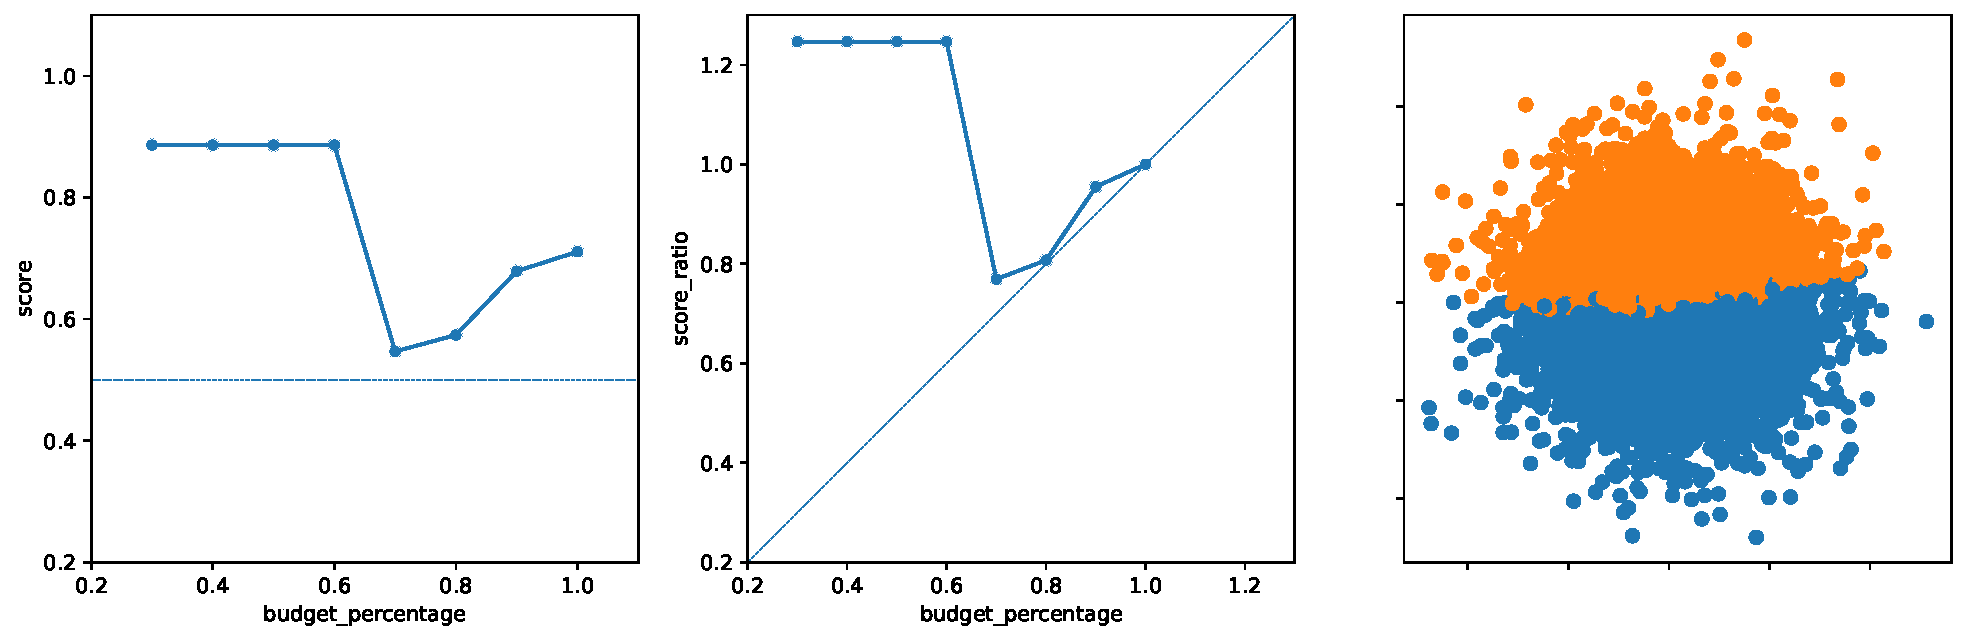
\includegraphics[width=\textwidth]{img/3d/1.pdf}
    \end{subfigure}%
    \hfill
    \begin{subfigure}{\textwidth}
        \centering
        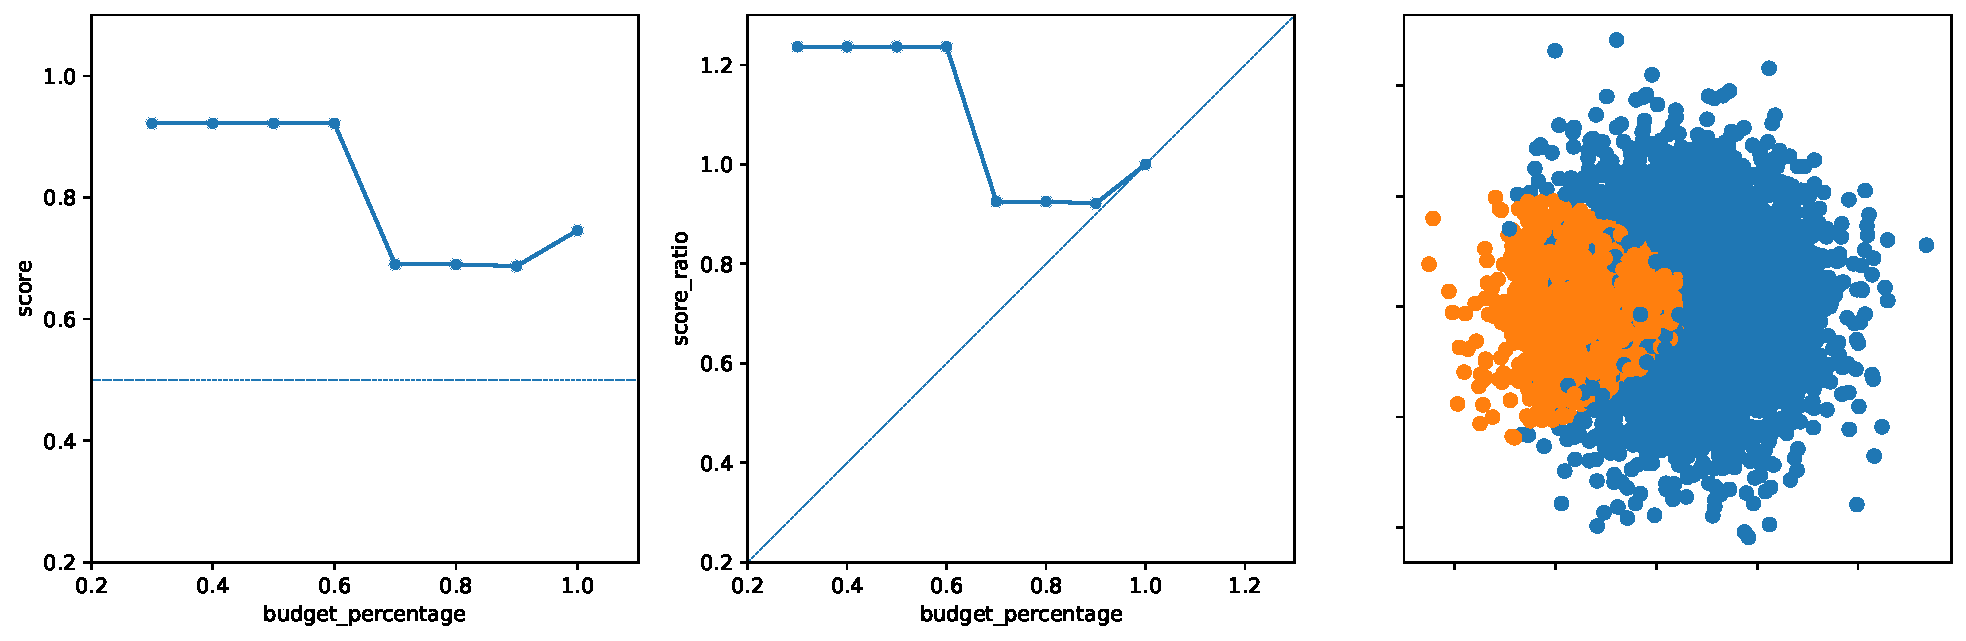
\includegraphics[width=\textwidth]{img/3d/2.pdf}
    \end{subfigure}%
    \hfill
    \begin{subfigure}{\textwidth}
        \centering
        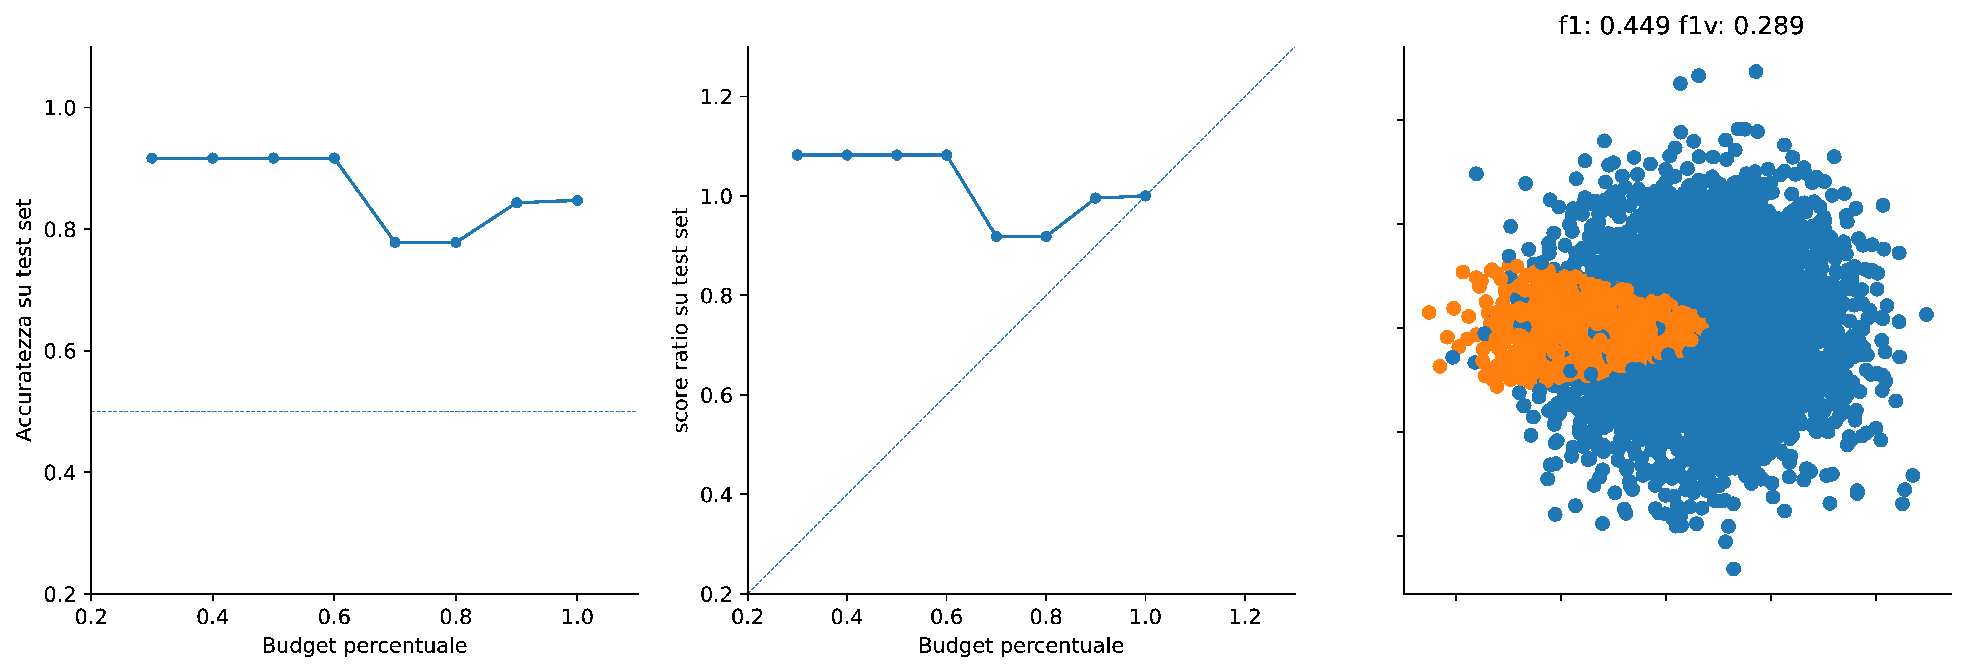
\includegraphics[width=\textwidth]{img/3d/3.pdf}
    \end{subfigure}%
\caption{Esperimenti su \emph{dataset} sintetici 3D utilizzando la strategia 1. A sinistra l'accuratezza sui dati di test al variare del \emph{budget}; al centro lo ``score ratio'' al variare del \emph{budget}; a destra il \emph{dataset} ridotto a due dimensioni utilizzando \emph{principal component analysis}.}
\label{fig:3d_exp}
\end{figure}
Dai risultati ottenuti si nota come per valori di \emph{budget} alti ($80/90\%$) l'andamento dei valori misurati sia in linea con le aspettative, calando proporzionalmente alla riduzione di \emph{budget}.
Tuttavia, l'accuratezza dei modelli con \emph{budget} più ristretti sale fino a superare l'accuratezza dei modelli classici, abbastanza bassa in termini assoluti.
Inoltre, i modelli classici utilizzano una quantità di vettori di supporto molto vicina alla dimensione dell'intero insieme di addestramento.
Questo comportamento è inatteso e meriterebbe un approfondimento futuro, non eseguito in questa tesi a causa dell'elevato tempo di calcolo richiesto per addestrare e selezionare i modelli.

\section{Esperimenti su dataset di terze parti}\label{sec:exp:real_ds}
Utilizzando i \emph{dataset} descritti nella~\Cref{tab:uci_datasets} sono stati effettuati degli esperimenti con le diverse strategie.

I risultati ottenuti utilizzando la strategia 1 sono illustrati in~\Cref{fig:TP_old_strategy}.
\begin{figure}
    \centering
    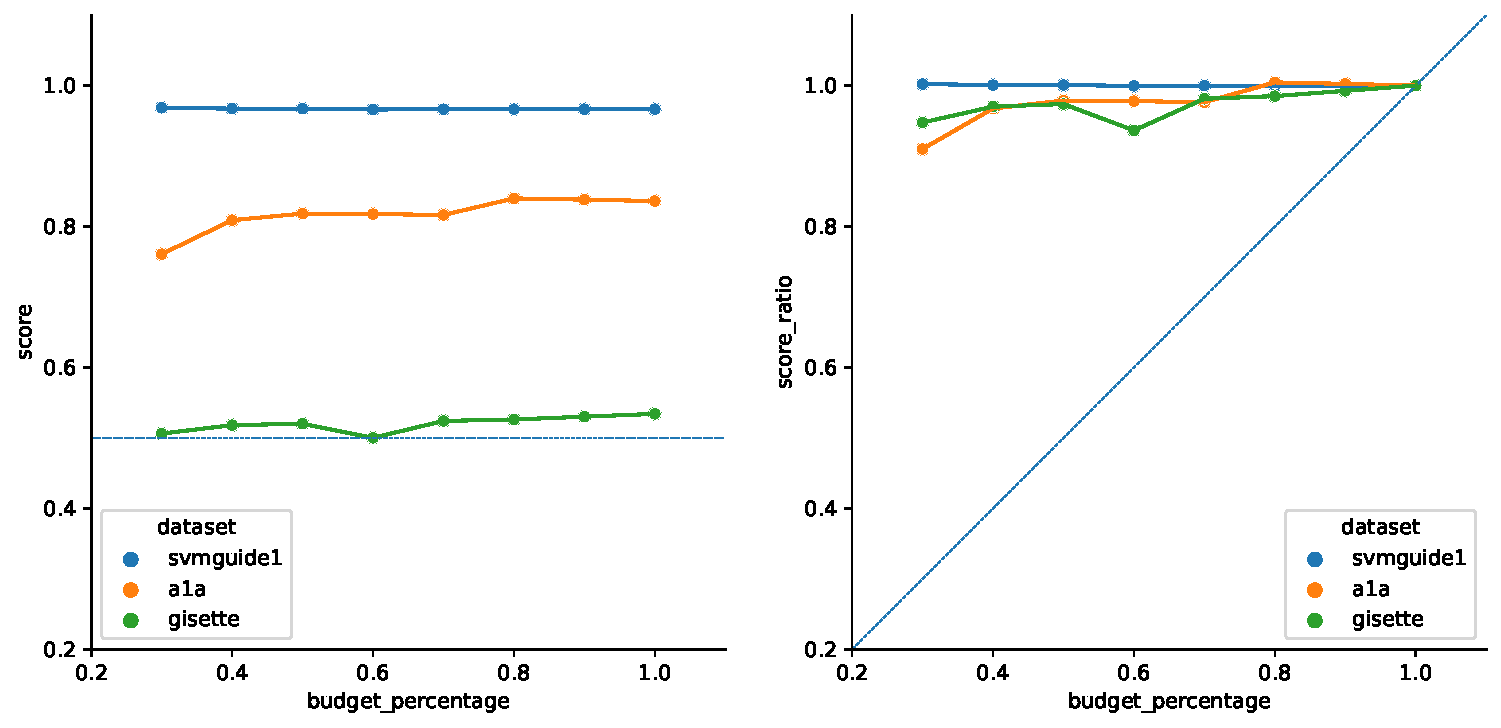
\includegraphics[width=1\linewidth]{img//TP/tp_old_strategy.pdf}
    \caption[Risultati su \emph{dataset} di terze parti utilizzando la strategia 1.]{Risultati esperimenti su \emph{dataset} di terze parti utilizzando la strategia 1. A sinistra l'accuratezza sui dati di test al variare del \emph{budget}; a destra lo \emph{score ratio} al variare del \emph{budget}.}
    \label{fig:TP_old_strategy}
\end{figure}
Si può notare come su questi \emph{dataset} tutte le riduzioni di \emph{budget} utilizzate siano efficaci e non risultino in perdite di accuratezza significative: ogni modello \emph{budgeted SVC} è sostanzialmente equivalente come bontà al rispettivo modello classico.
L'accuratezza ottenuta sul \emph{dataset gisette} indica come nessuno dei modelli prodotti sia efficace a modellare quel problema; questo risultato non è preoccupante perché le caratteristiche di questi dati rendono il problema particolarmente difficile: questo \emph{dataset} è di dimensione modesta (6000 elementi di addestramento) rispetto al numero degli attributi (5000).

I risultati ottenuti utilizzando la strategia 2 sono illustrati in~\Cref{fig:TP_new_strategy}.
\begin{figure}
    \centering
    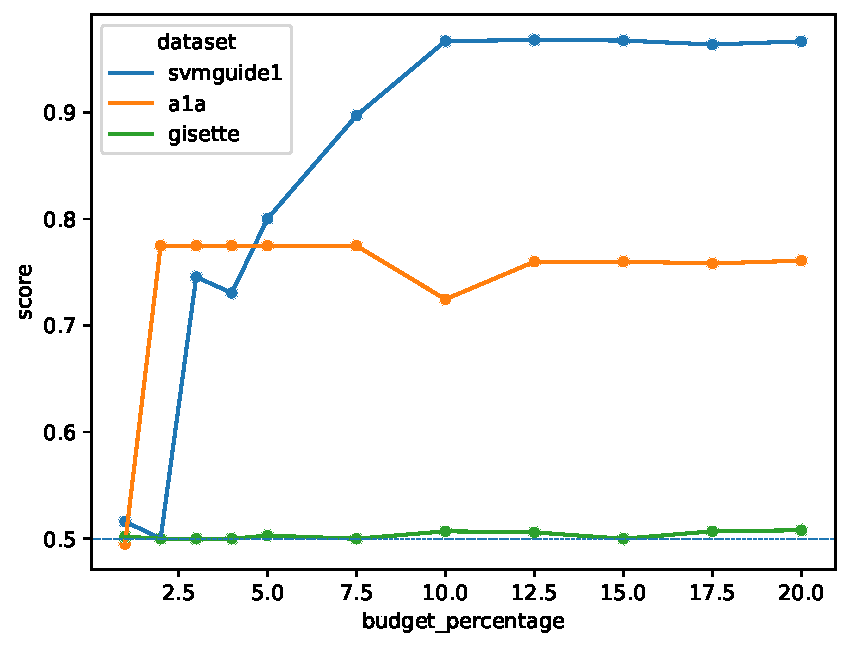
\includegraphics[width=0.5\linewidth]{img//TP/tp_new_strategy.pdf}
    \caption[Risultati su \emph{dataset} di terze parti utilizzando la strategia 2.]{Accuratezza al variare del \emph{budget} sui \emph{dataset} di terze parti utilizzando la strategia 2.}
    \label{fig:TP_new_strategy}
\end{figure}
Così come per gli analoghi esperimenti effettuati su \emph{dataset} sintetici, è possibile notare come per ogni \emph{dataset} sia possibile identificare un valore soglia di \emph{budget} che divide \emph{budget} non penalizzanti da \emph{budget} penalizzanti.

\section{Comparazione con altri metodi}\label{sec:comparazione_metodi}
Per meglio inquadrare i risultati ottenuti dal metodo \emph{budgeted SVC}, son stati ripetuti gli esperimenti descritti in precedenza utilizzando delle implementazioni di metodi proposti in letteratura e descritti nel~\Cref{chap:sparse_svc}, in particolare:
\begin{itemize}
    \item \emph{BSGD SVM}~\cite{2012_bsgd}, risolutore pensato per addestramento \emph{on-line} basato su discesa del gradiente che mantiene una dimensione massima dell'insieme dei vettori di supporto utilizzando la strategia di unione o rimozione;
    \item \emph{NSSVM}~\cite{2020_sparse_svm}, risolutore basato su \emph{Newton method} che minimizza il numero di vettori di supporto tramite una funzione di costo adatta.
    % \item \emph{LIB IRWLS} esposto in~\cite{LIBIRWLS}. Risolutore parallelo basato su un approssimazione \emph{greedy} della matrice \emph{kernel} e utilizzo dell'algoritmo IRWLS~\cite{IRWLS}
\end{itemize}
Utilizzando gli stessi \emph{dataset} sintetici generati con i parametri nelle~\Cref{tab:parametri_ds_sin,tab:parametri_ds_pacman} e utilizzando \emph{5-fold cross-validation} con una ricerca estensiva sulla griglia di parametri adatti in~\Cref{tab:gridsearch_comparazioni}, viene misurata l'accuratezza sui dati di \emph{test} per gli stessi valori di \emph{budget} utilizzati negli esperimenti precedenti.
\begin{table}
    \centering
    \begin{tabular}{ccccc}
        \toprule
        Algoritmo & $C$ & \emph{Kernel} & $\gamma$ & d \\
        \midrule
        \multirow{2}{*}{BSGD}   & \multirow{2}{*}{/}  & Gaussiano   & [0.001, 0.01, 0.1, 1, 10]   & /\\
                                      \cline{3-5}
                                &   & Polinomiale & / & [2, 5, 10] \\
        \hline
        NSSVM   & / & / & / & / \\
        % \hline
        % IRWLS   & [0.01, 0.1, 1, 10]  & Gaussiano & [0.001, 0.01, 0.1, 1, 10] & / \\
        \bottomrule
    \end{tabular}
    \caption{Parametri \emph{grid search} per gli algoritmi presenti in letteratura.}
    \label{tab:gridsearch_comparazioni}
\end{table}
In~\Cref{fig:comp_old} si possono vedere i risultati ottenuti utilizzando la strategia 1, mentre in~\Cref{fig:comp_new} si possono vedere i risultati ottenuti utilizzando la strategia 2.
Come per gli esperimenti precedenti queste figure riportano i risultati più significativi, mentre i restanti grafici sono inseriti nell'Appendice A.
\begin{figure}
    \begin{subfigure}{.5\textwidth}
        \centering
        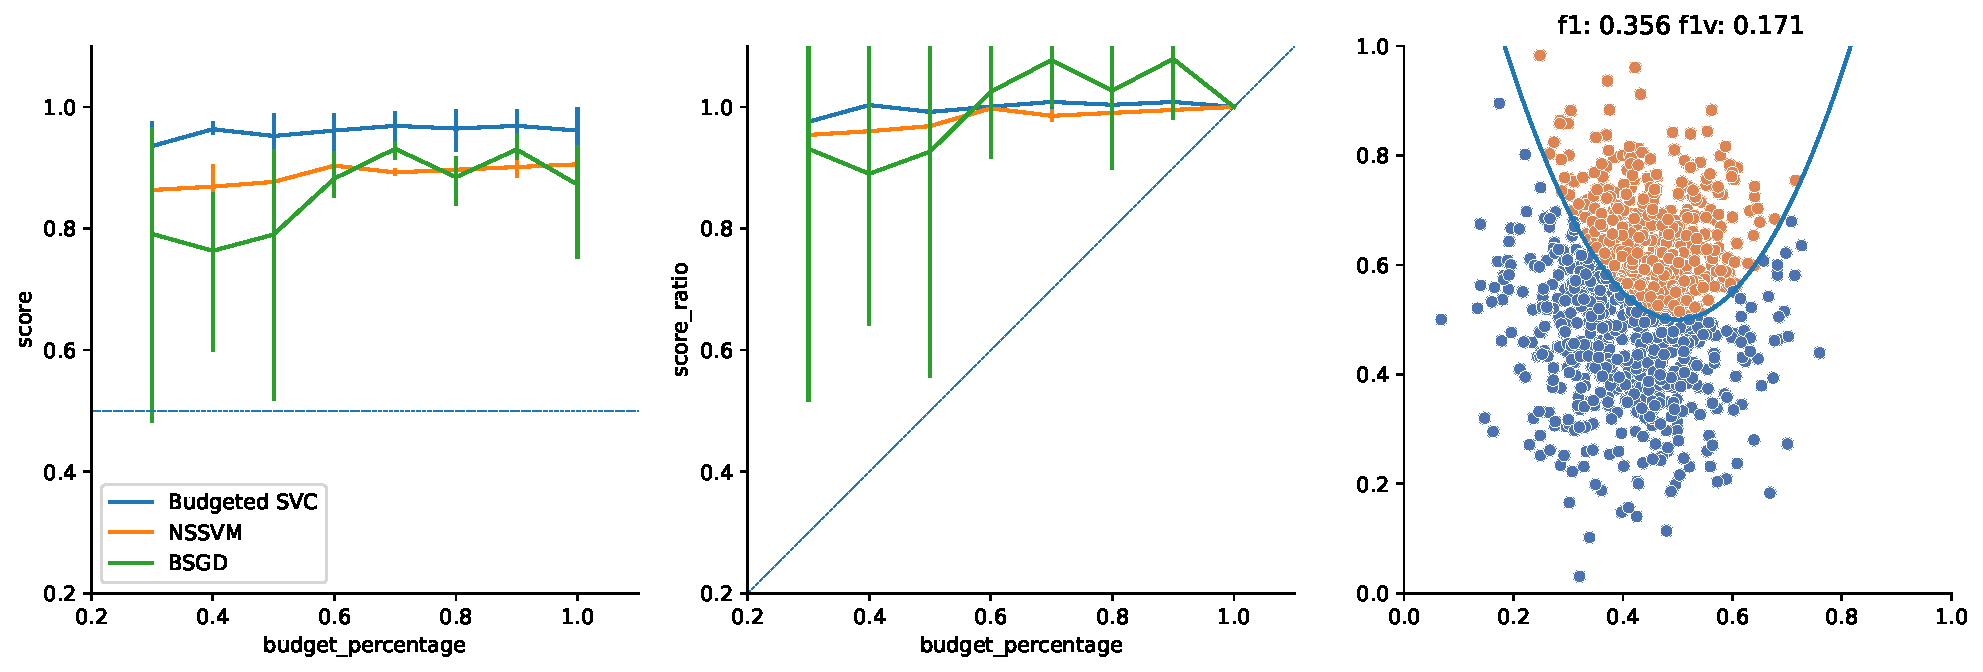
\includegraphics[width=\textwidth]{img/comp_old/3.pdf}
    \end{subfigure}%
    \begin{subfigure}{.5\textwidth}
        \centering
        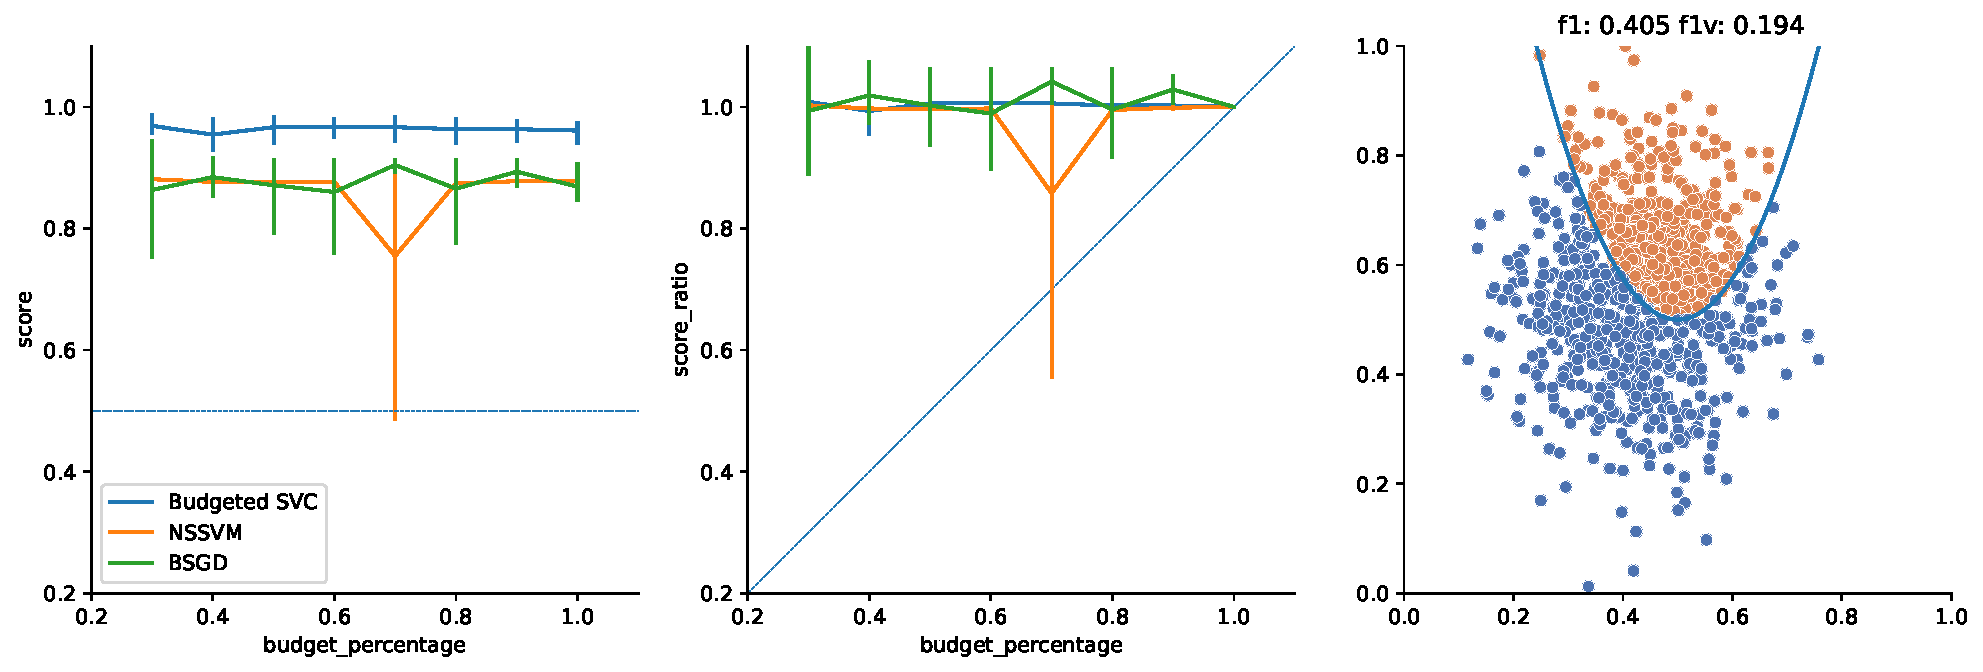
\includegraphics[width=\textwidth]{img/comp_old/4.pdf}
    \end{subfigure}
    %
    \hfill
    %
    \begin{subfigure}{.5\textwidth}
        \centering
        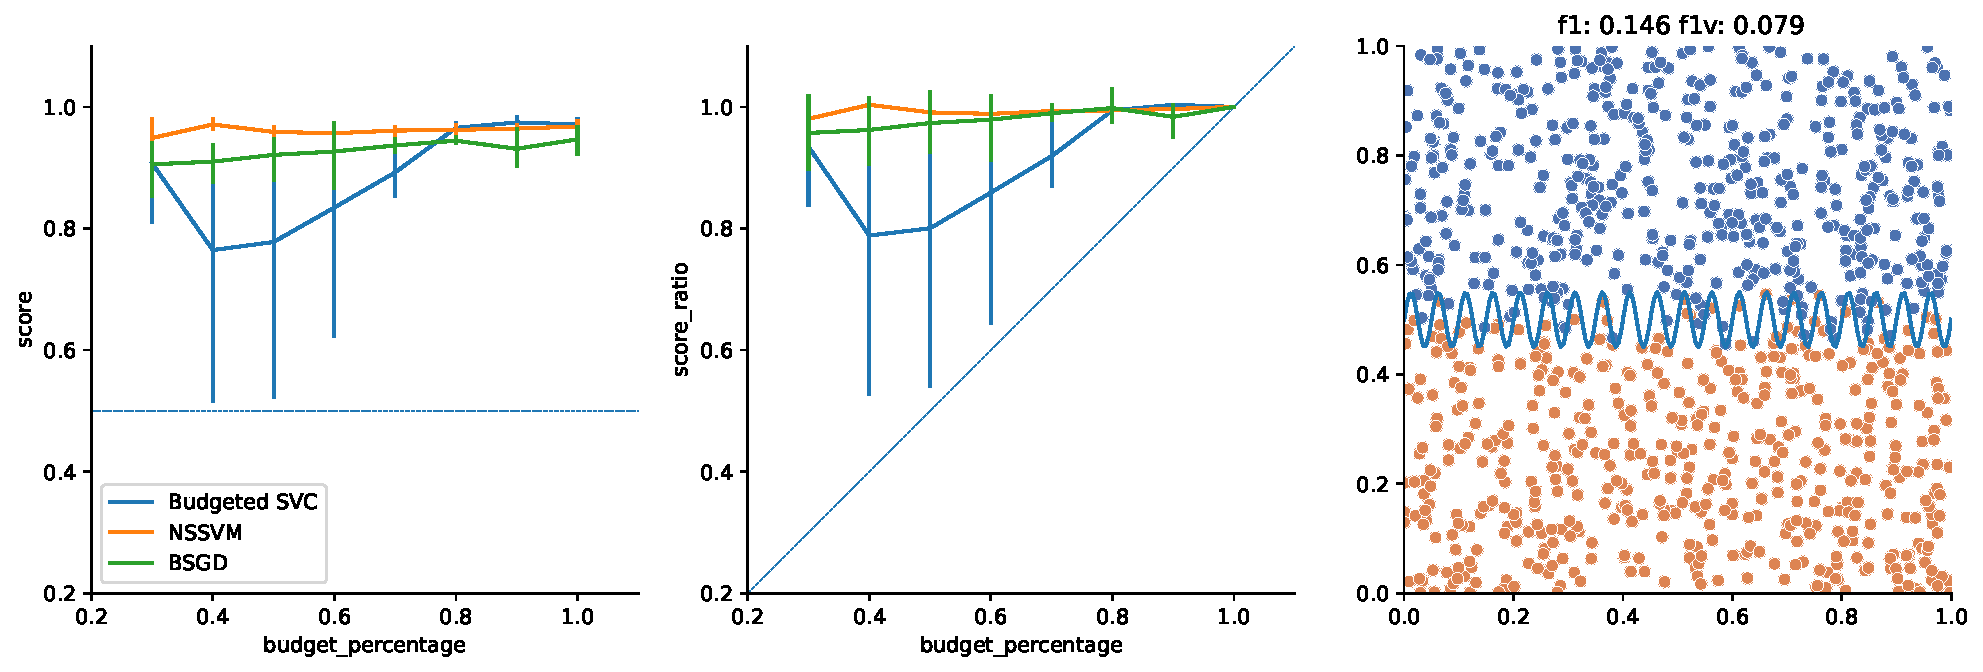
\includegraphics[width=\textwidth]{img/comp_old/8.pdf}
    \end{subfigure}
    \begin{subfigure}{.5\textwidth}
        \centering
        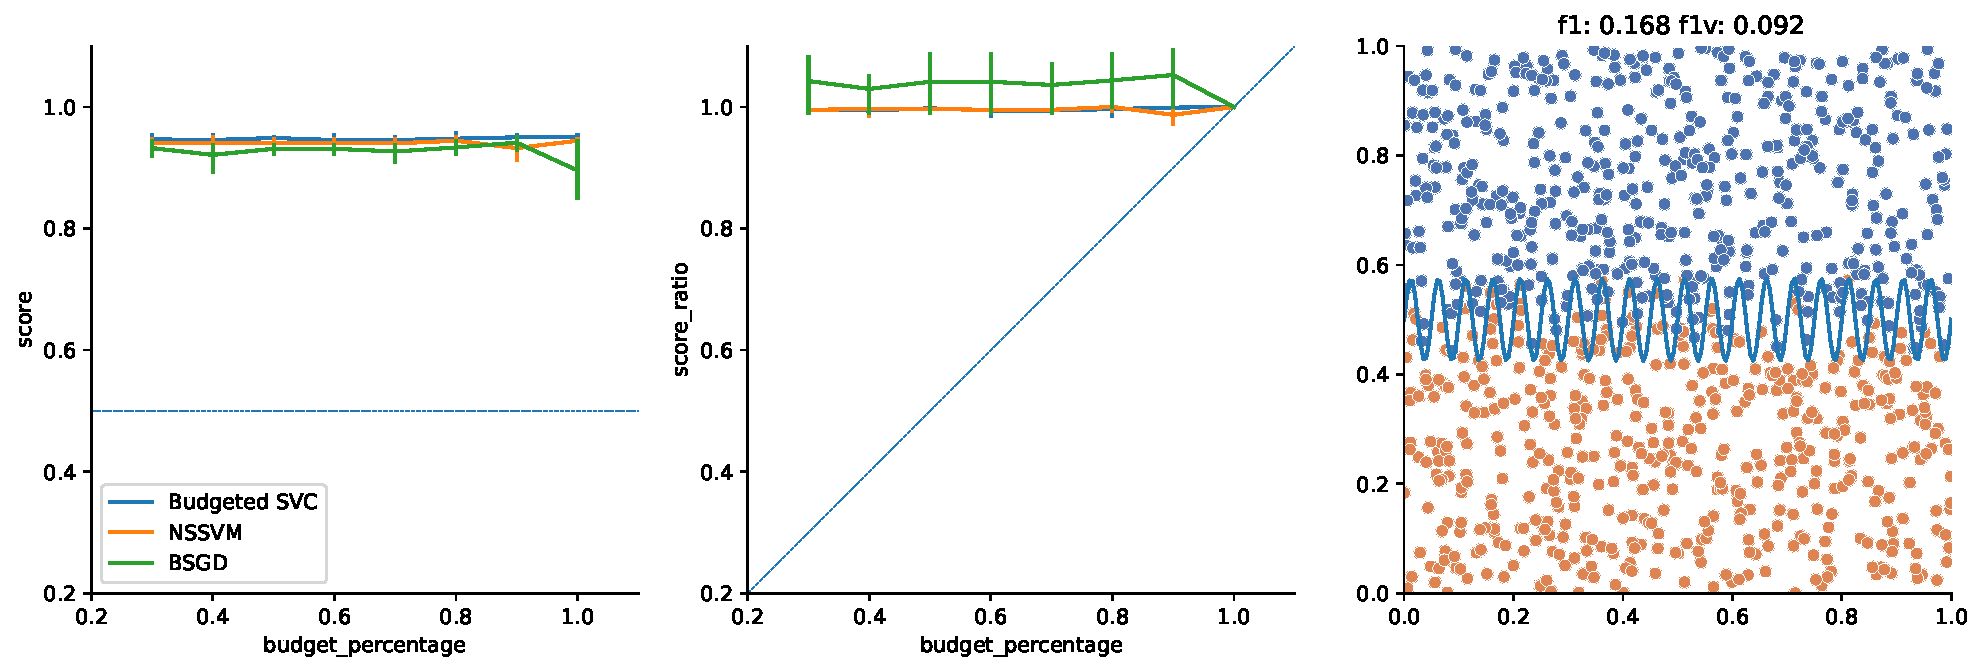
\includegraphics[width=\textwidth]{img/comp_old/9.pdf}
    \end{subfigure}%
    %
    \hfill
    %
    \begin{subfigure}{.5\textwidth}
        \centering
        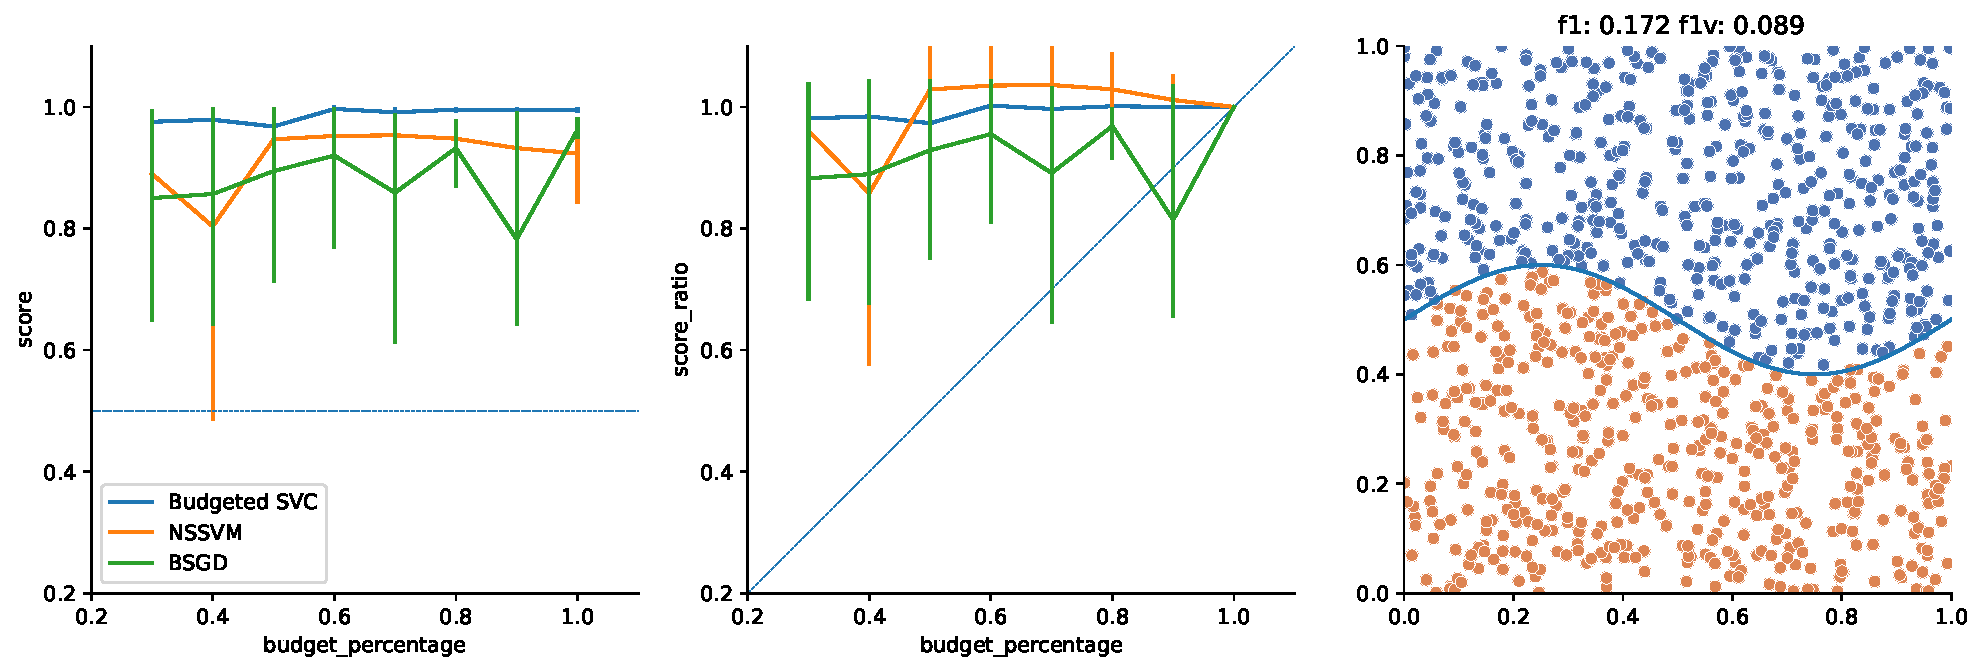
\includegraphics[width=\textwidth]{img/comp_old/10.pdf}
    \end{subfigure}
    \begin{subfigure}{.5\textwidth}
        \centering
        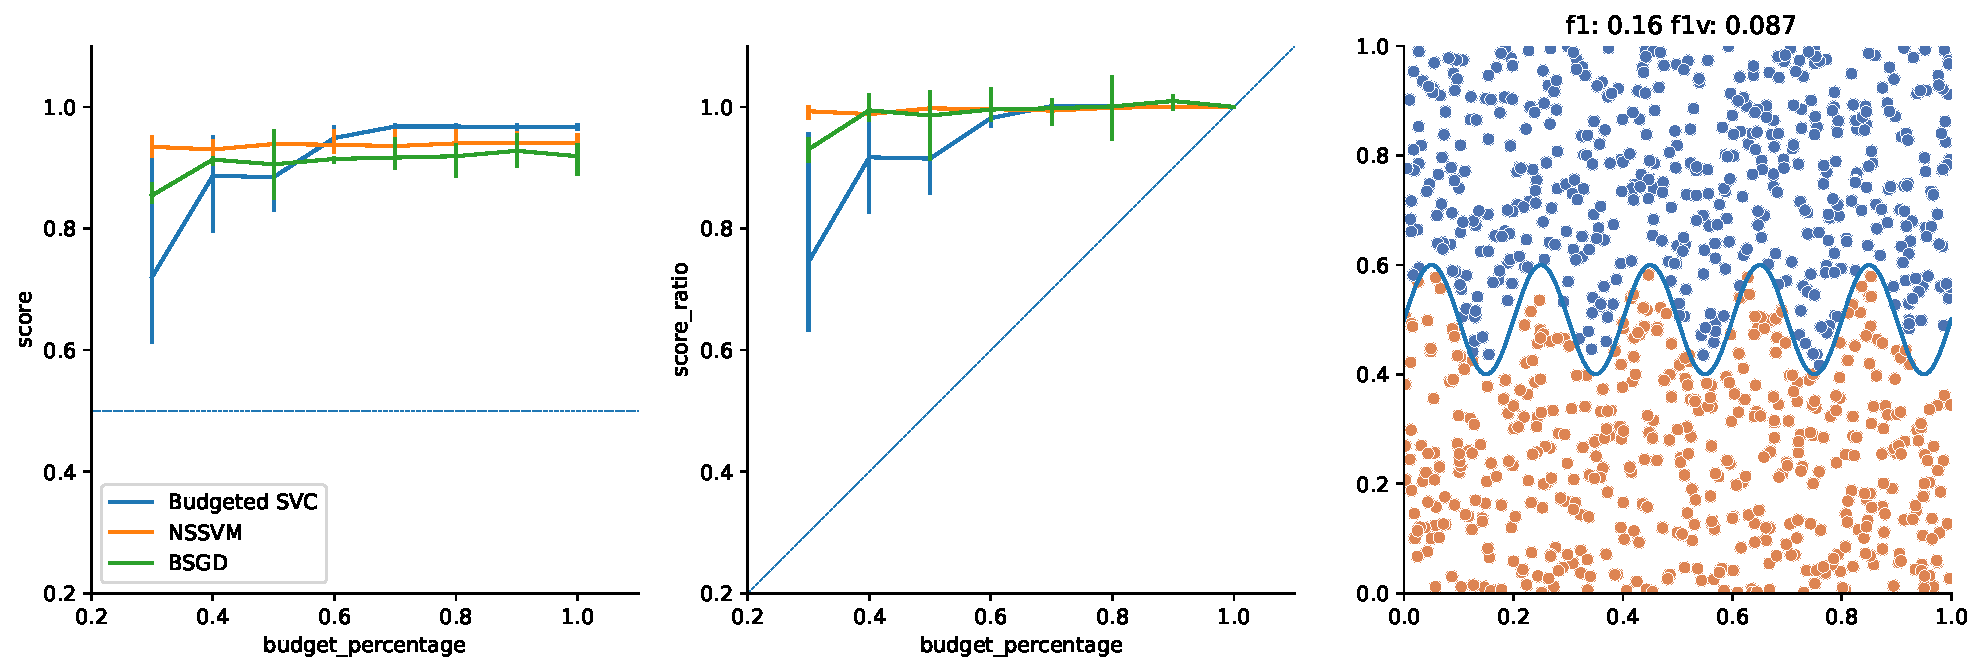
\includegraphics[width=\textwidth]{img/comp_old/12.pdf}
    \end{subfigure}%
    %
    \hfill
    %
    \begin{subfigure}{.5\textwidth}
        \centering
        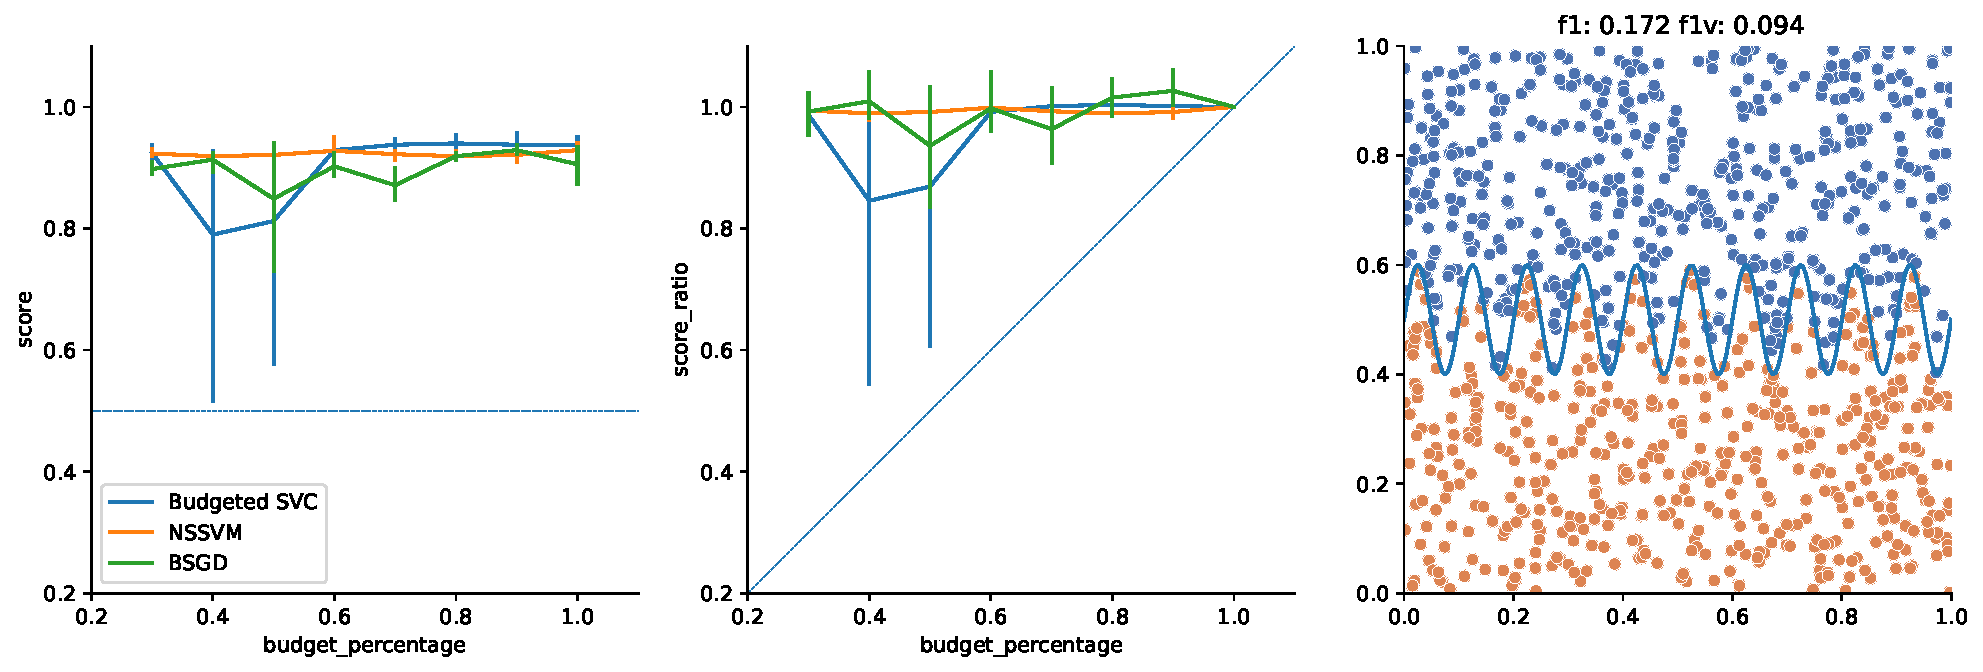
\includegraphics[width=\textwidth]{img/comp_old/13.pdf}
    \end{subfigure}
    \begin{subfigure}{.5\textwidth}
        \centering
        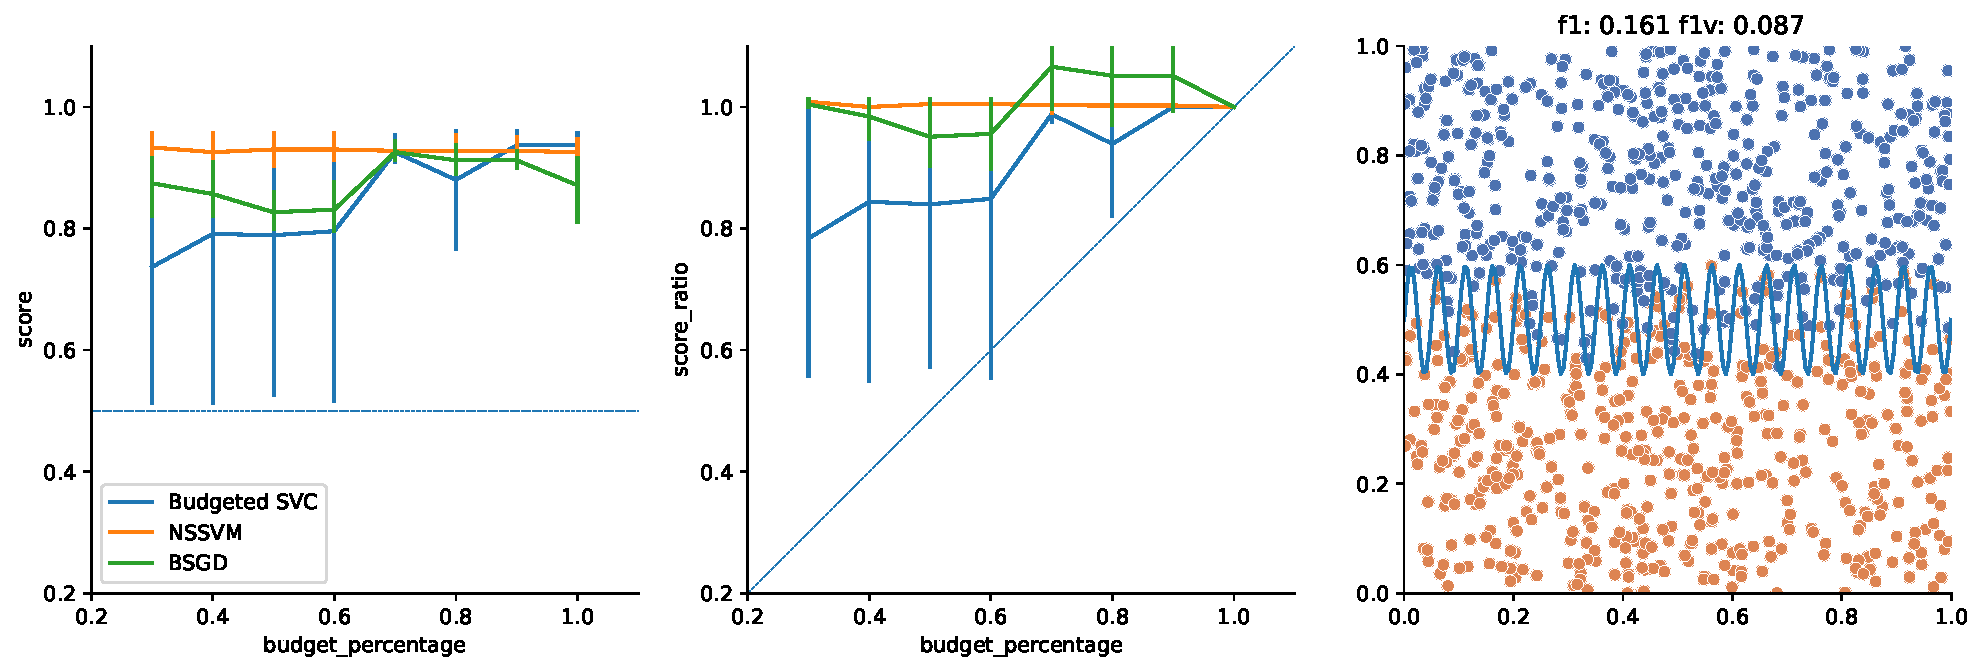
\includegraphics[width=\textwidth]{img/comp_old/14.pdf}
    \end{subfigure}
        %
    \hfill
    %
    \begin{subfigure}{.5\textwidth}
        \centering
        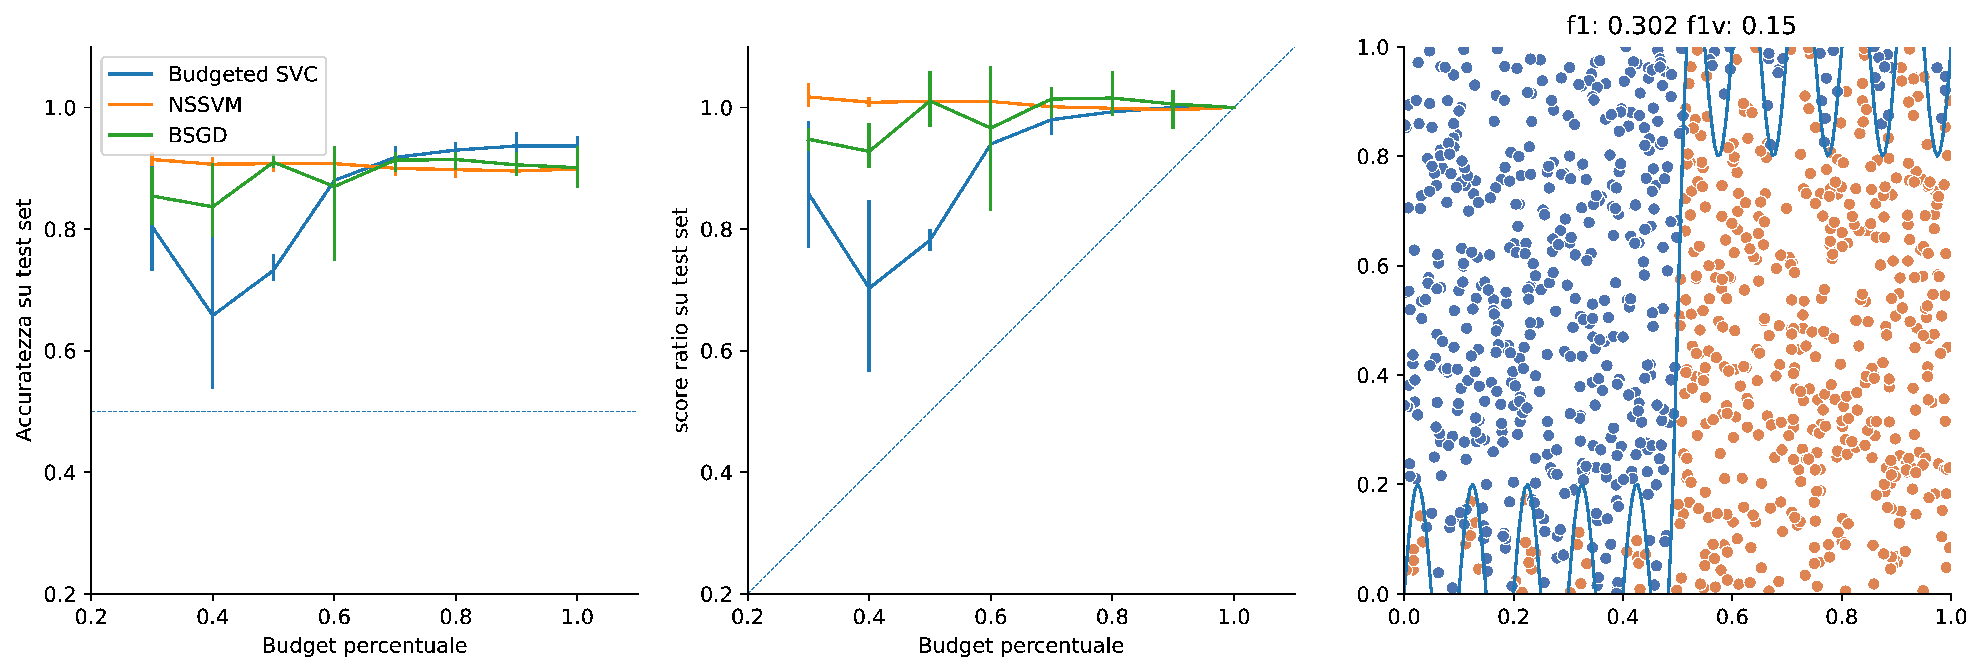
\includegraphics[width=\textwidth]{img/comp_old/15.pdf}
    \end{subfigure}
\caption[Risultati su \emph{dataset} sintetici utilizzando strategia 1 in confronto ad altri metodi.]{Risultati più significativi ottenuti su \emph{dataset} sintetici 2D utilizzando la strategia 1, analogo ai risultati in~\Cref{fig:risultati_2d} ma con una curva per ogni metodo utilizzato: la proposta \emph{Budgeted SVC}, i metodi \emph{NSSVM} e \emph{BSGD}.}
\label{fig:comp_old}
\end{figure}
Confrontando i risultati ottenuti con la strategia 1, è possibile notare come anche i modelli prodotti dagli altri metodi, con frequenza minore, risultino in valori di accuratezza molto vari per i diversi \emph{dataset} generati con seme diverso.
Allo stesso tempo, escludendo pochi casi anomali, la perdita di accuratezza al variare di \emph{budget} ottenuta da questi metodi sembra essere più lineare rispetto alla proposta \emph{budgeted SVC}.
\begin{figure}
    \begin{subfigure}{.5\textwidth}
        \centering
        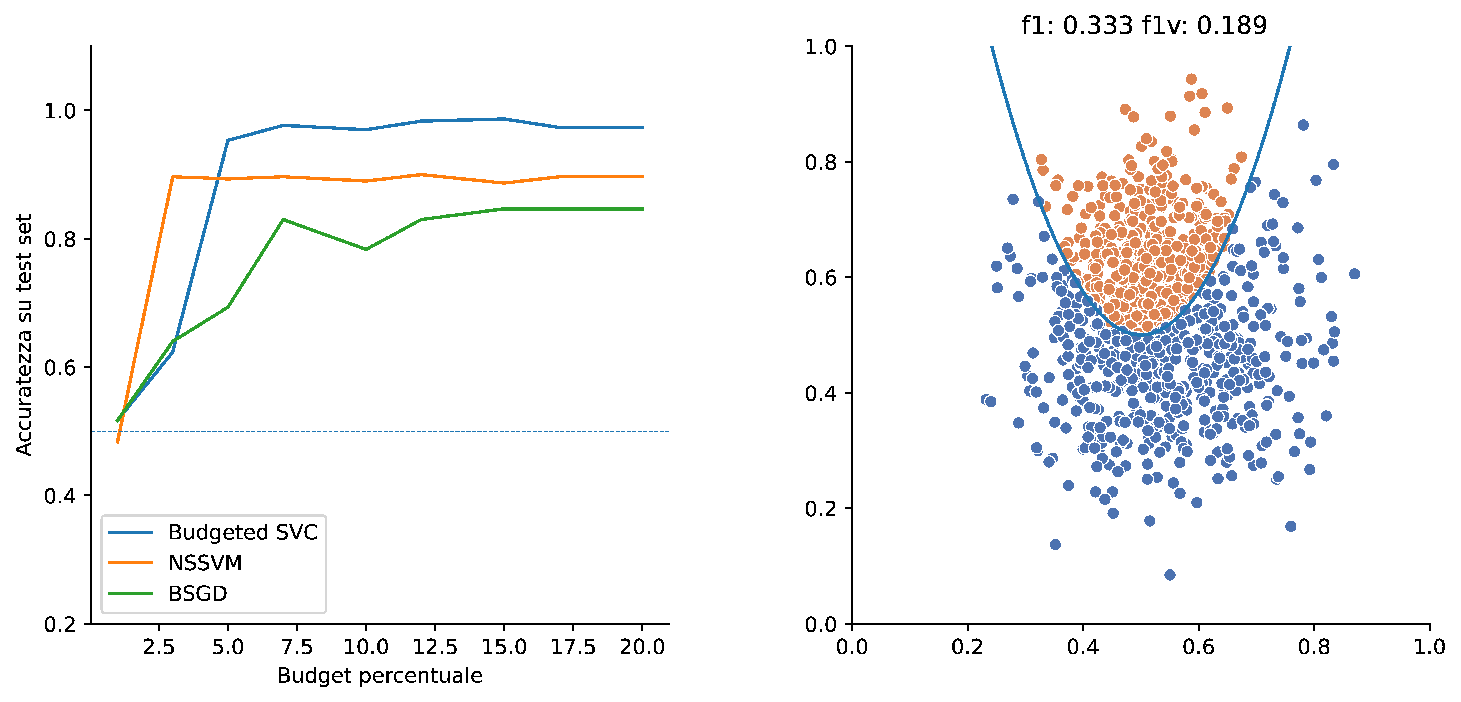
\includegraphics[width=\textwidth]{img/comp_new/4.pdf}
    \end{subfigure}%
    \begin{subfigure}{.5\textwidth}
        \centering
        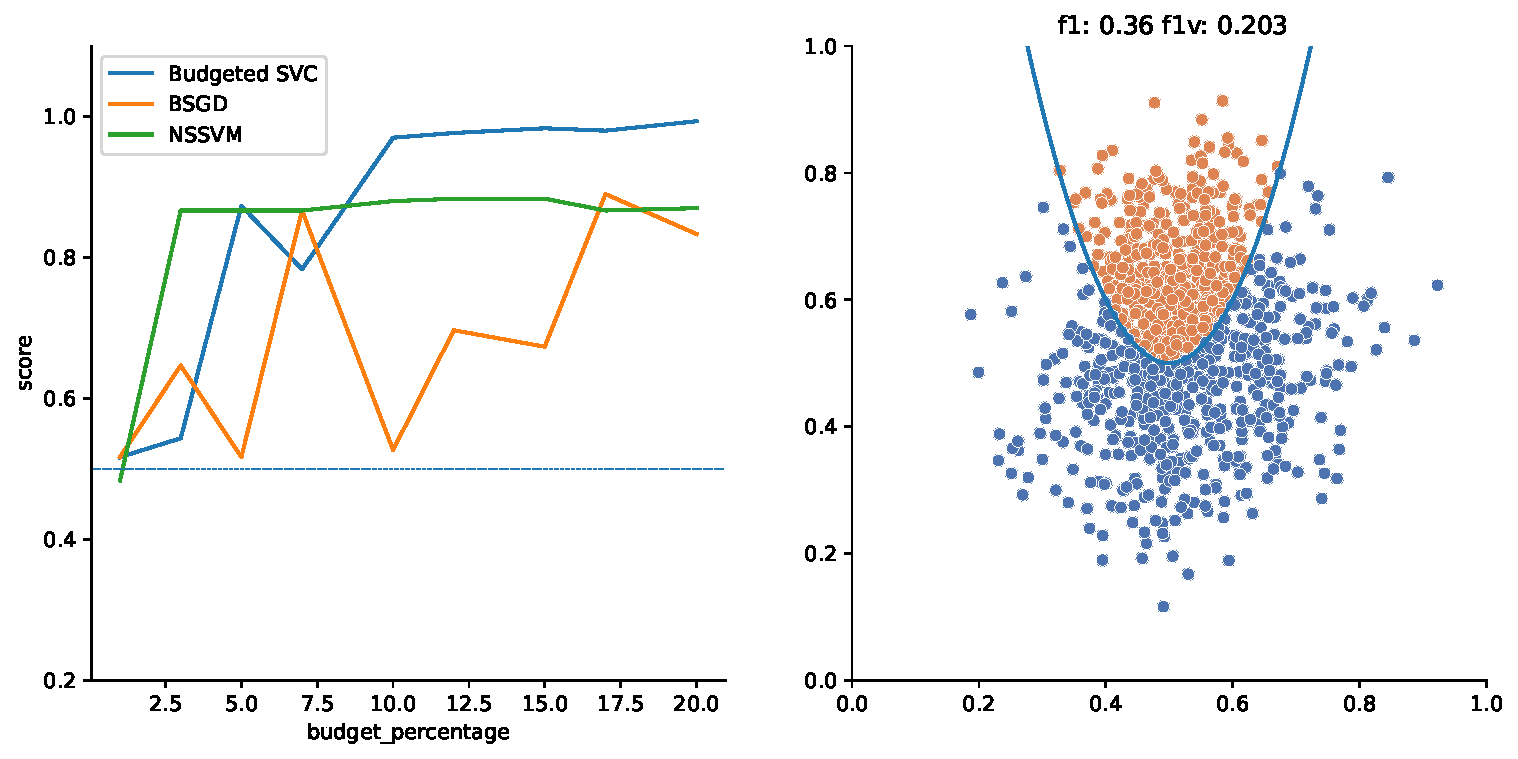
\includegraphics[width=\textwidth]{img/comp_new/5.pdf}
    \end{subfigure}
    %
    \hfill
    %
    \begin{subfigure}{.5\textwidth}
        \centering
        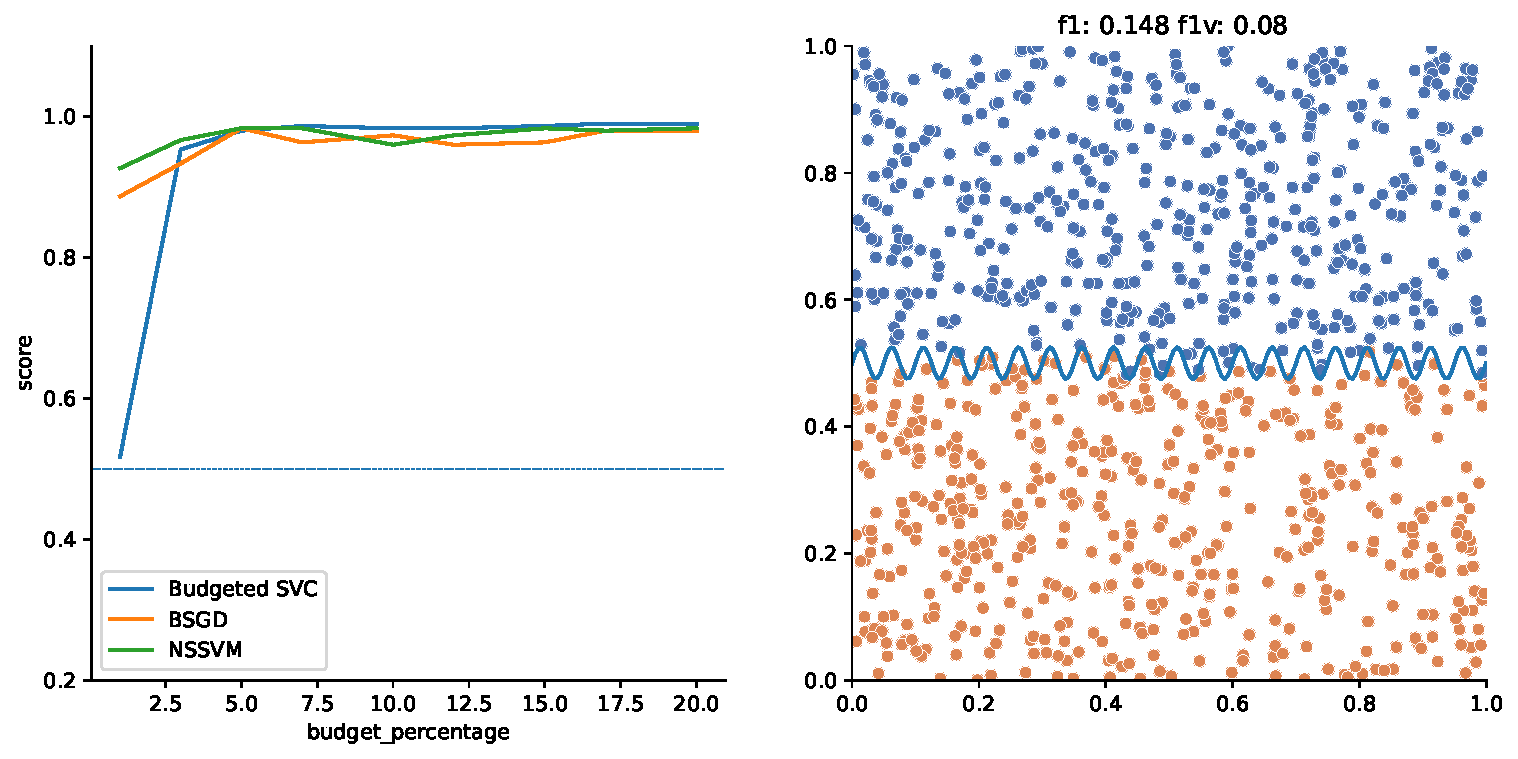
\includegraphics[width=\textwidth]{img/comp_new/7.pdf}
    \end{subfigure}
    \begin{subfigure}{.5\textwidth}
        \centering
        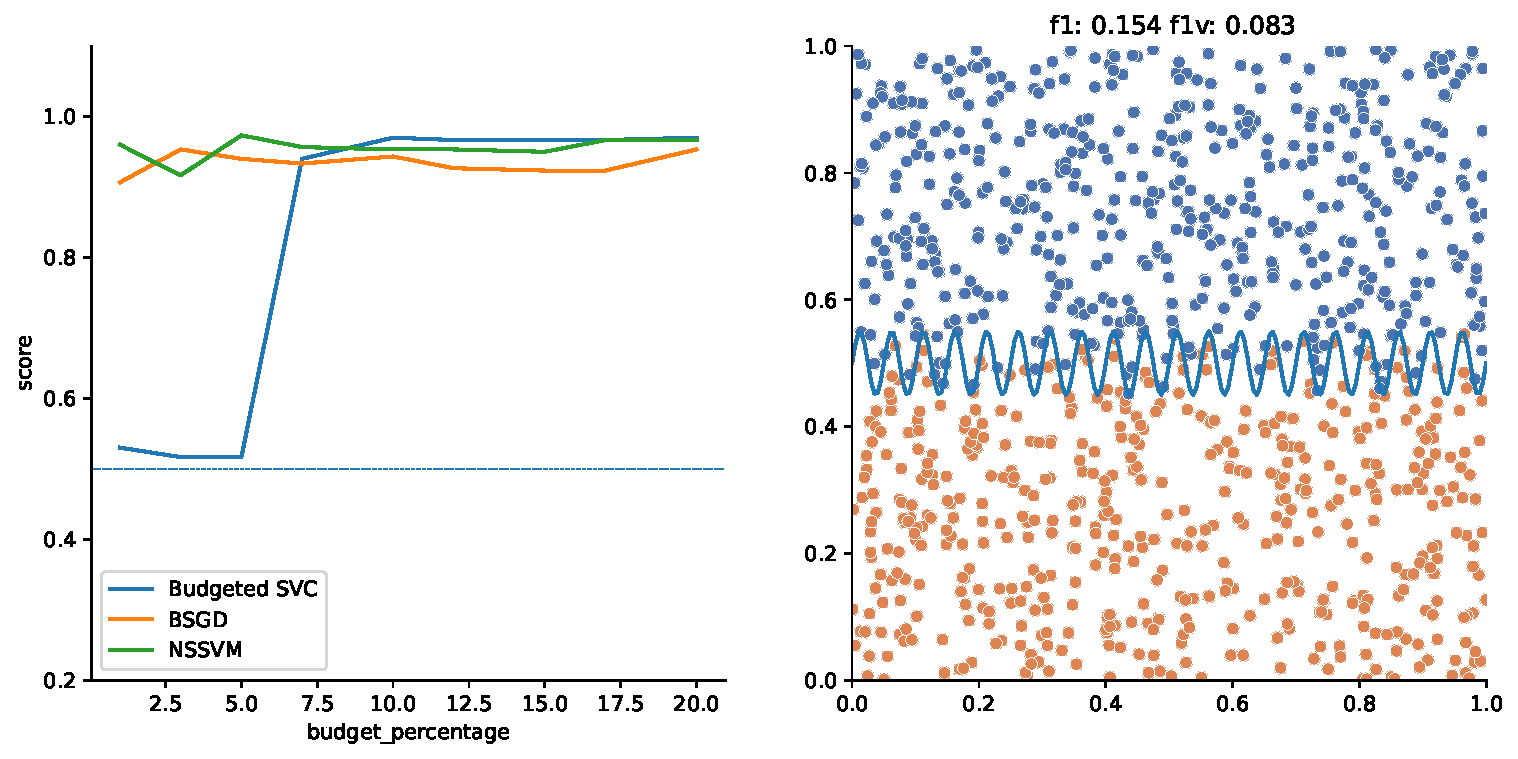
\includegraphics[width=\textwidth]{img/comp_new/8.pdf}
    \end{subfigure}%
    %
    \hfill
    %
    \begin{subfigure}{.5\textwidth}
        \centering
        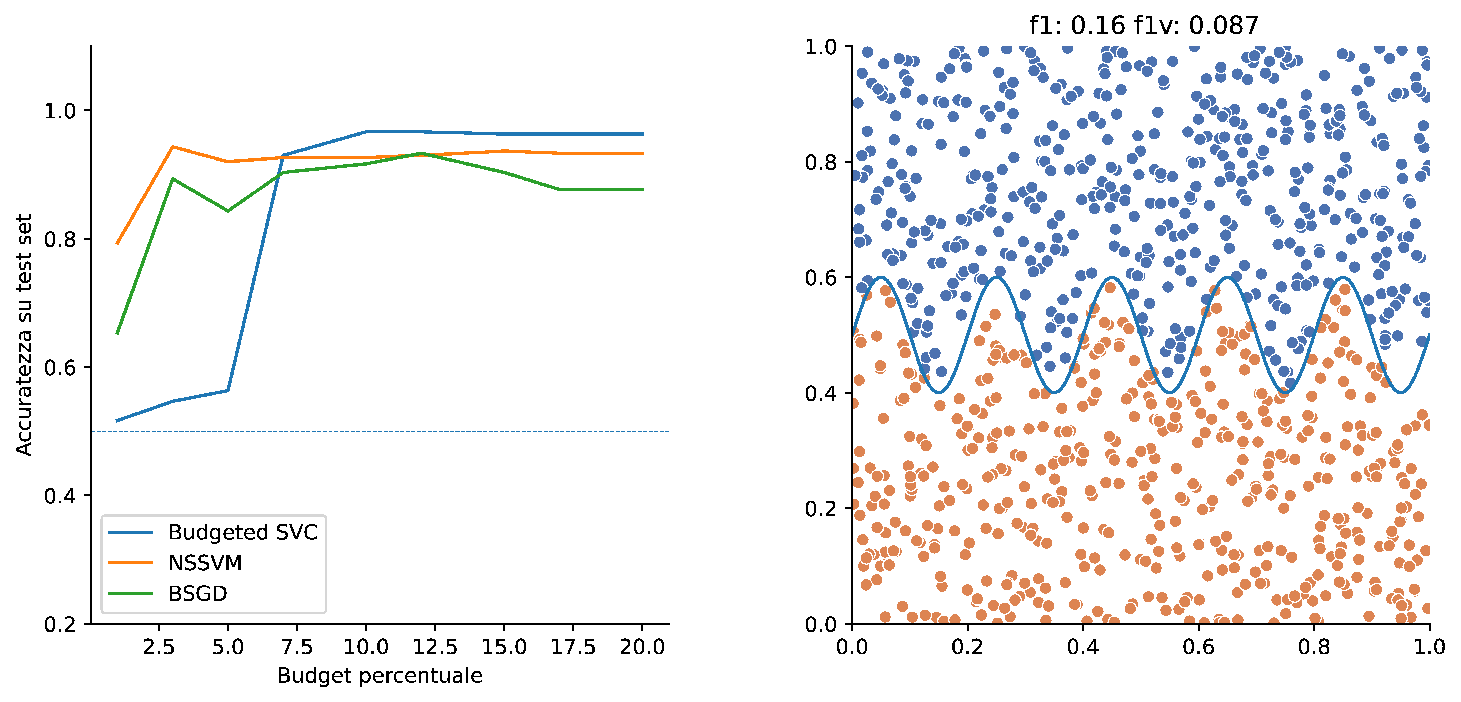
\includegraphics[width=\textwidth]{img/comp_new/12.pdf}
    \end{subfigure}
    \begin{subfigure}{.5\textwidth}
        \centering
        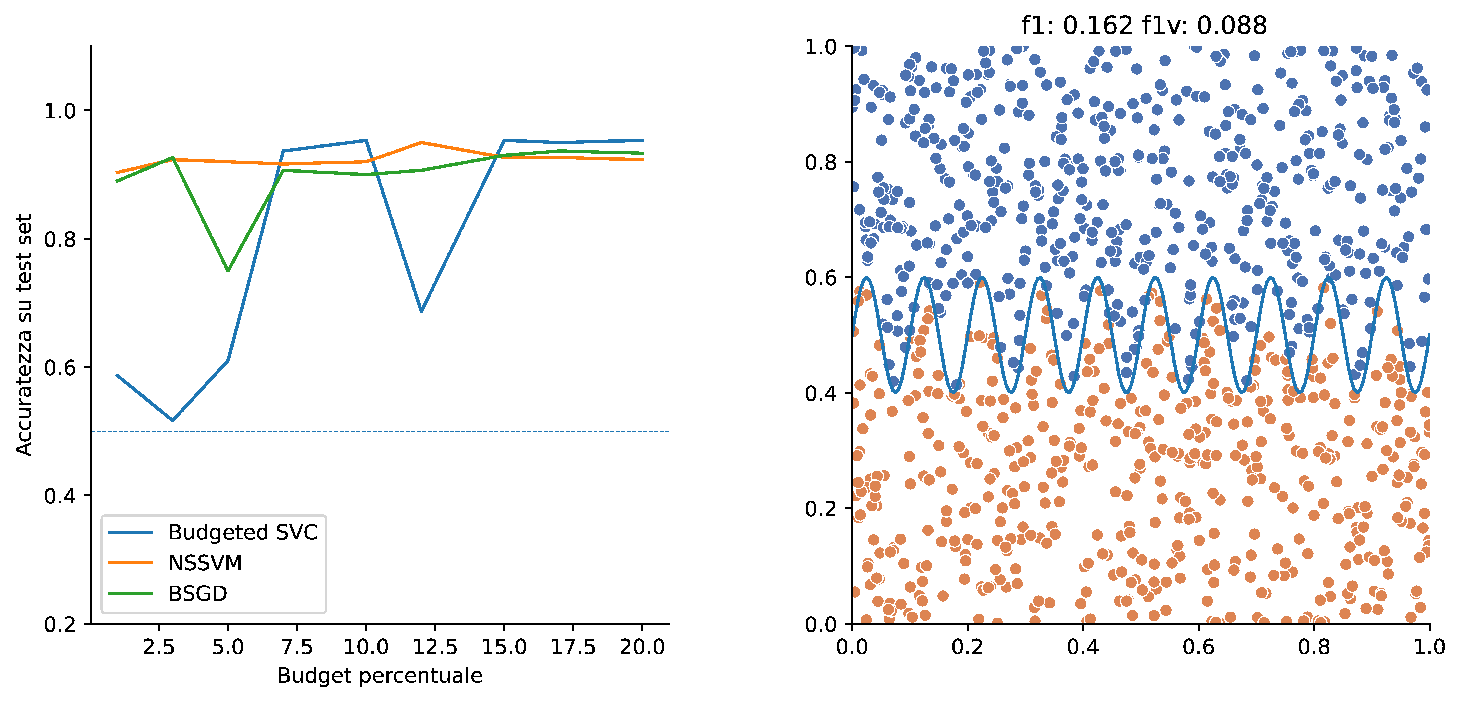
\includegraphics[width=\textwidth]{img/comp_new/13.pdf}
    \end{subfigure}%
    %
    \hfill
    %
    \begin{subfigure}{.5\textwidth}
        \centering
        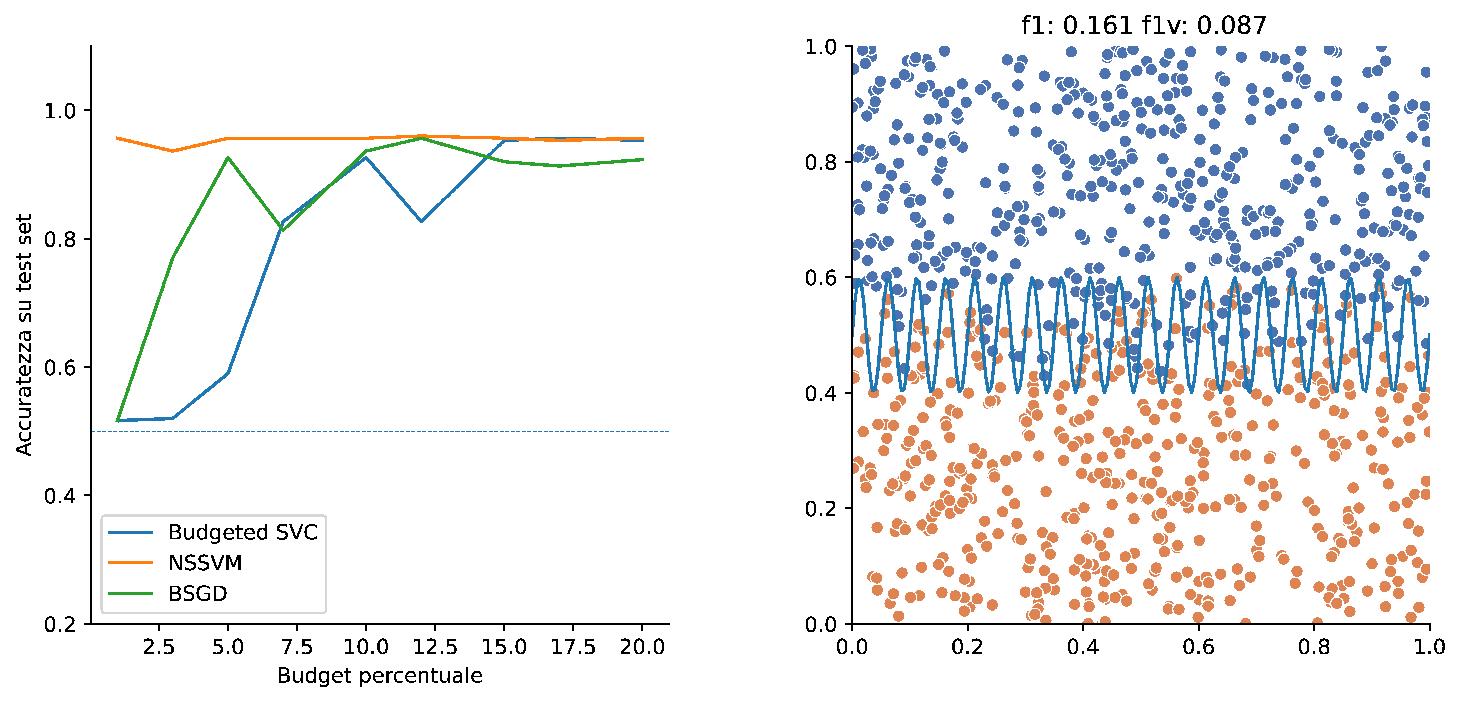
\includegraphics[width=\textwidth]{img/comp_new/14.pdf}
    \end{subfigure}
    \begin{subfigure}{.5\textwidth}
        \centering
        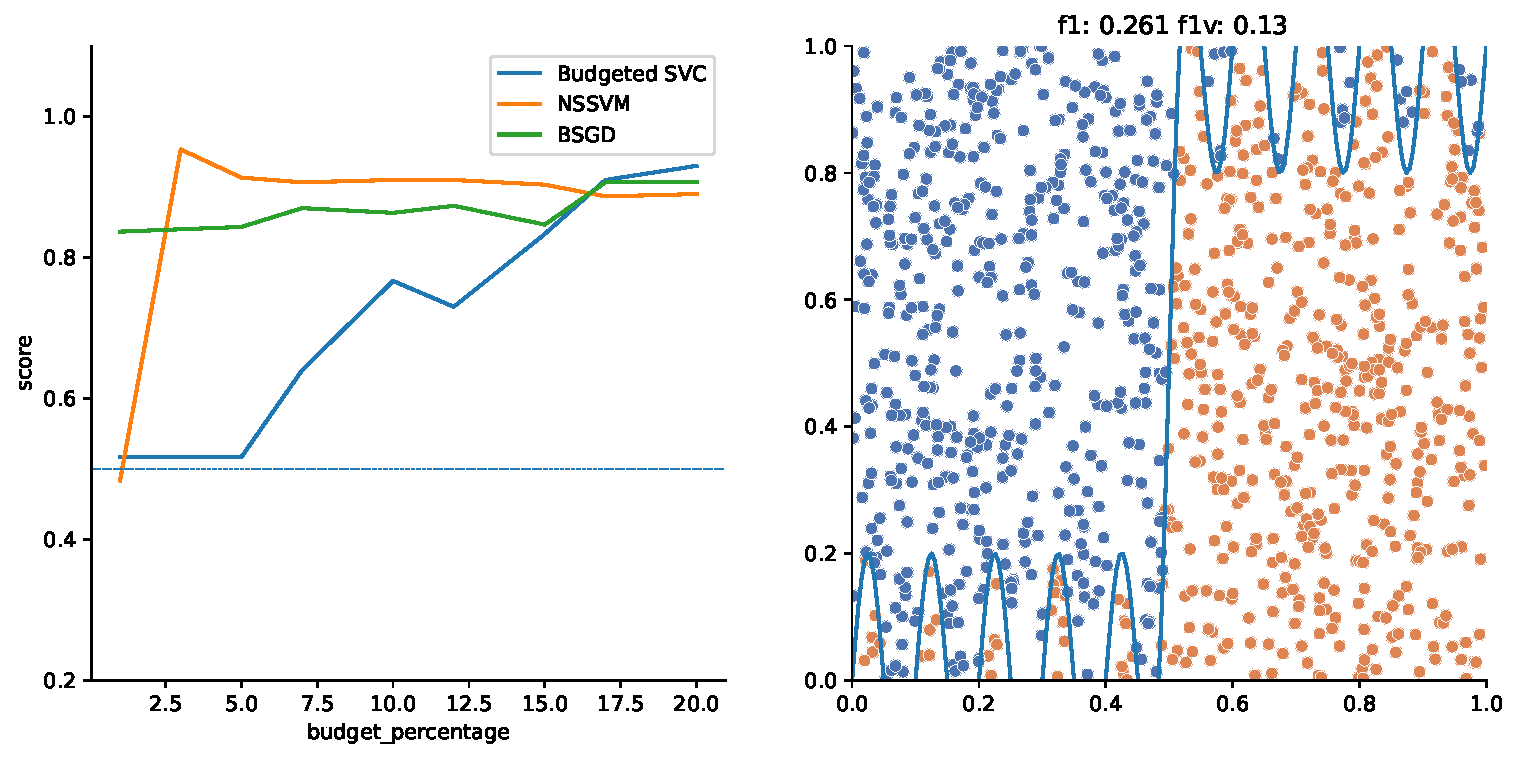
\includegraphics[width=\textwidth]{img/comp_new/15.pdf}
    \end{subfigure}
\caption[Risultati su \emph{dataset} sintetici utilizzando strategia 2 in confronto ad altri metodi.]{Risultati più significativi ottenuti su \emph{dataset} sintetici 2D utilizzando la strategia 2, analogo ai risultati in~\Cref{fig:2d_v2} ma con una curva per ogni metodo utilizzato: la proposta \emph{Budgeted SVC}, i metodi \emph{NSSVM} e \emph{BSGD}.}
\label{fig:comp_new}
\end{figure}
Confrontando i risultati ottenuti con la strategia 2, si può notare come i modelli prodotti dalla formulazione \emph{budgeted SVC} siano competitivi per valori di \emph{budget} alti e come siano invece peggiori per valori di \emph{budget} bassi. 
La perdita di accuratezza dovuta alla restrizione di \emph{budget} si manifesta per \emph{budgeted SVC} con valori di \emph{budget} più alti rispetto agli altri metodi.

\section{Memorizzazione compressa dei modelli SVC}\label{sec:memorizzazione_compressa}
Un ulteriore metodo per diminuire lo spazio di memorizzazione richiesto per un modello SVC si basa sull'osservazione che, nella formulazione \emph{soft margin}, i moltiplicatori $\alpha_i$ sono al più grandi quanto $C$, e non è quindi necessario memorizzare tutti i moltiplicatori $\alpha_i = C$.

Assumendo che le etichette positive abbiano valore $+1$ e le etichette negative abbiano valore $-1$ (e considerando che si può sempre forzare questa assunzione a essere vera), si definiscono i valori:
\begin{itemize}
    \item $s^+ = |\{\alpha_i, i=1,\dots,m : 0 < \alpha_i < C, y_i=+1\}|$ il numero di moltiplicatori con valore compreso in $(0, C)$ e con etichetta appartenente alla classe positiva;
    \item $s^- = |\{\alpha_i, i=1,\dots,m : 0 < \alpha_i < C, y_i=-1\}|$ il numero di moltiplicatori con valore compreso in $(0, C)$ e con etichetta appartenente alla classe negativa;
    \item $b^+ = |\{\alpha_i, i=1,\dots,m : \alpha_i = C, y_i=+1\}|$ il numero di moltiplicatori con valore uguale a $C$ e con etichetta appartenente alla classe positiva;
    \item $b^- = |\{\alpha_i, i=1,\dots,m : \alpha_i = C, y_i=-1\}|$ il numero di moltiplicatori con valore uguale a $C$ e con etichetta appartenente alla classe negativa.
\end{itemize}
Si ipotizzi quindi di memorizzare i vettori di supporto in gruppi contigui in base alla valore dei corrispettivi moltiplicatori, utilizzando l'ordinamento rappresentato in~\Cref{fig:schema_memorizzazione_sv}.
\begin{figure}
    \centering
    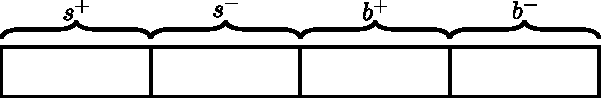
\includegraphics{img/memorizzazione_sv.pdf}
    \caption{Esempio di memorizzazione ordinata dei vettori di supporto. Ogni gruppo (identificato da un rettangolo) contiene vettori di supporto i quali moltiplicatori appartengono alla stessa categoria.}
    \label{fig:schema_memorizzazione_sv}
\end{figure}
Utilizzando questa memorizzazione compressa, l'originale calcolo di una nuova predizione per il punto $\Vec{x}_{\text{test}}$
\begin{equation*}
    h(\Vec{x}_{\text{test}}) = \sign\left(\sum_{i \in S}\alpha_i^*y_iK(\Vec{x}_i, \Vec{x}_\text{test}) + b^*\right),
\end{equation*}
visto nel~\Cref{sec:kernel_trick}, può essere trasformato in
\begin{align*}
    h(\Vec{x}_{\text{test}}) = \sign\bigg(
            \sum_{i=1}^{s^+}\alpha_i^*K(\Vec{x}_i, \Vec{x}_\text{test}) 
            -\sum_{i=s^+}^{s^-}\alpha_i^*K(\Vec{x}_i, \Vec{x}_\text{test})\\
            +C\sum_{i=s^-}^{b^+}K(\Vec{x}_i, \Vec{x}_\text{test})
            -C\sum_{i=b^+}^{b^-}K(\Vec{x}_i, \Vec{x}_\text{test}) 
            + b^*
        \bigg).
\end{align*}
Si può notare come questa rappresentazione compressa sia vantaggioso in termini di spazio, perché non è necessario memorizzare tutti i moltiplicatori lagrangiani con valore uguale a $C$.
D'altra parte, si complica leggermente la realizzazione pratica del modello.
In~\Cref{tab:compressione_spazio_risparmiato} si confrontano i requisiti di spazio per una memorizzazione classica e la memorizzazione compressa.
\begin{table}
    \centering
    \begin{tabular}{c|c|c}
    \multicolumn{1}{c}{}    &  Memorizzazione Classica    & Memorizzazione Compressa \\     
    \toprule
    Numero di moltiplicatori    & $s^+ + s^- + b^+ + b^-$ & $s^+ +s^-$ \\
    \hline
    Numero di etichette         & $s^+ + s^- + b^+ + b^-$ &  / \\
    \hline
    Altre variabili             &         $b^*$          &  $s^+, s^-, b^+, b^-, C, b^*$ \\
    \bottomrule
    \end{tabular}
    \caption{Requisiti di spazio della memorizzazione classica e delle memorizzazione compressa.}
    \label{tab:compressione_spazio_risparmiato}
\end{table}
Come si può notare, la memorizzazione compressa consente di evitare di memorizzare $b^++b^-$ moltiplicatori rispetto alla memorizzazione classica.
Ipotizzando che i moltiplicatori siano variabili \emph{float} da quattro \emph{byte} ciascuna, si possono risparmiare $4(b^++b^-)$ \emph{byte} relativamente ai moltiplicatori lagrangiani e $4(s^+ + s^- + b^+ + b^-)$ relativamente alle etichette, ma sono richieste cinque variabili intere aggiuntive per memorizzare $s^+, s^-, b^+, b^-, C$.
La memorizzazione compressa è praticamente sempre conveniente in termini di spazio, ed è tanto più conveniente quanto la quantità $b^++b^-$ è grande.

Per avere delle indicazioni di quanto spazio si possa risparmiare utilizzando questa rappresentazione, si mostrano nelle~\Cref{fig:dist_riduzione_synth_old,fig:dist_riduzione_synth_new} le distribuzioni delle potenziali riduzioni in spazio richiesto per memorizzare gli indici per gli esperimenti su \emph{dataset} sintetici descritti nel~\Cref{sec:exp:synth_2d} e si mostrano nelle~\Cref{fig:dist_riduzione_TP_old,fig:dist_riduzione_TP_new} le distribuzioni delle potenziali riduzioni in spazio richiesto per memorizzare gli indici per gli esperimenti su \emph{dataset} di terze parti descritti nel~\Cref{sec:exp:real_ds}.
\begin{figure}
    \centering
    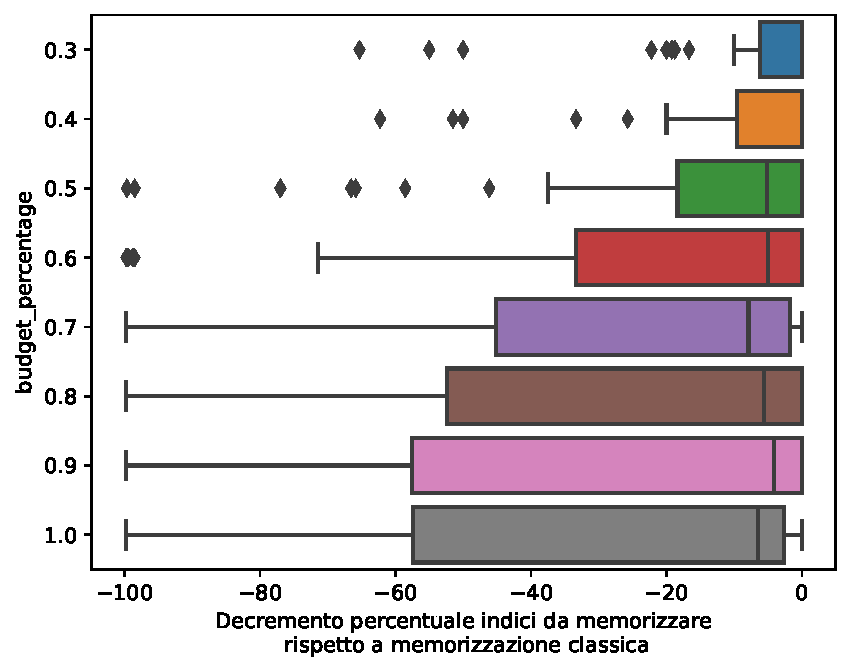
\includegraphics[width=.7\linewidth]{img/decremento_spazio_indici_exp2d_old.pdf}
    \caption{Distribuzioni, per percentuale di \emph{budget}, della riduzione dello spazio richiesto per memorizzare gli indici, relativamente agli esperimenti su \emph{dataset} sintetici effettuati con strategia 1.}
    \label{fig:dist_riduzione_synth_old}
\end{figure}%
\begin{figure}
    \centering
    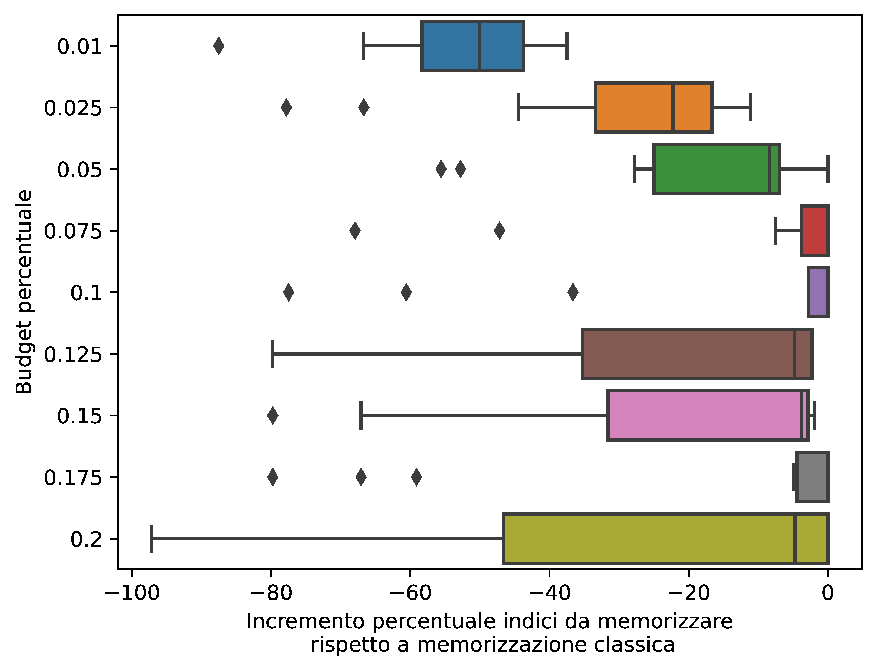
\includegraphics[width=.7\linewidth]{img/decremento_spazio_indici_exp2d_new.pdf}
    \caption{Distribuzioni, per percentuale di \emph{budget}, della riduzione dello spazio richiesto per memorizzare gli indici, relativamente agli esperimenti su \emph{dataset} sintetici effettuati con strategia 2.}
    \label{fig:dist_riduzione_synth_new}
\end{figure}
\begin{figure}
    \centering
    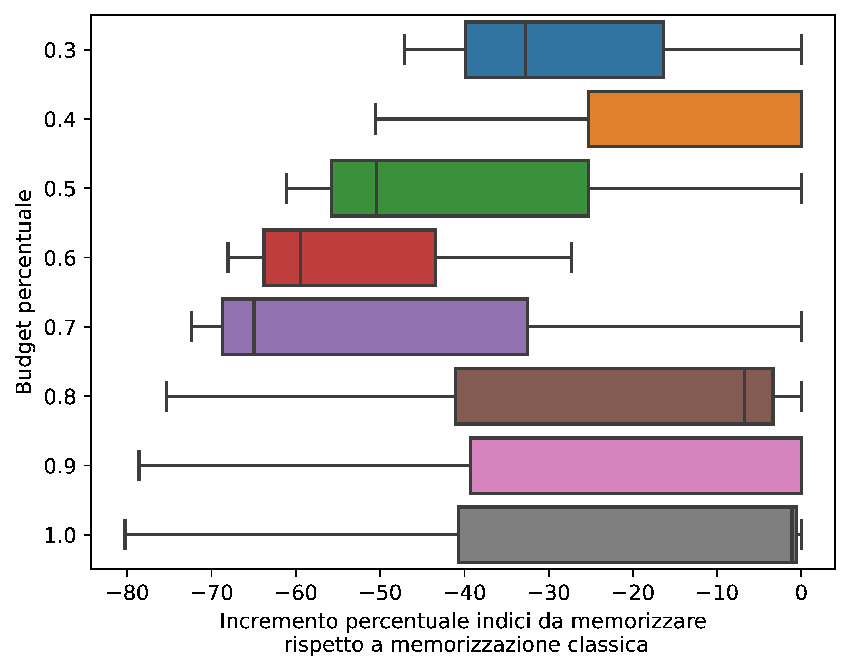
\includegraphics[width=.7\linewidth]{img/decremento_spazio_indici_TP_old.pdf}
    \caption{Distribuzioni, per percentuale di \emph{budget}, della riduzione dello spazio richiesto per memorizzare gli indici, relativamente agli esperimenti su \emph{dataset} di terze parti effettuati con strategia 1.}
    \label{fig:dist_riduzione_TP_old}
\end{figure}%
\begin{figure}
    \centering
    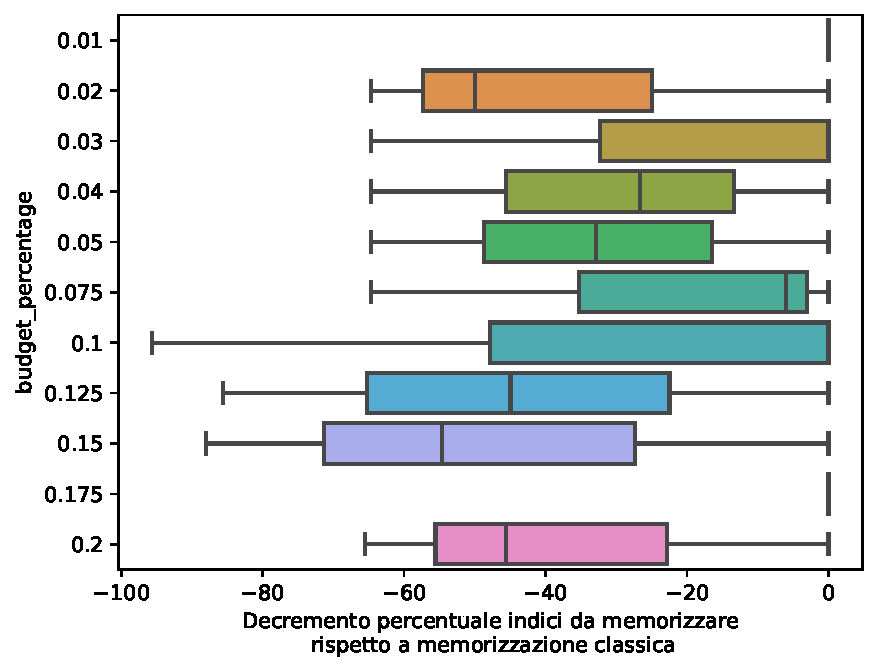
\includegraphics[width=.7\linewidth]{img/decremento_spazio_indici_TP_new.pdf}
    \caption{Distribuzioni, per percentuale di \emph{budget}, della riduzione dello spazio richiesto per memorizzare gli indici, relativamente agli esperimenti su \emph{dataset} di terze parti effettuati con strategia 2.}
    \label{fig:dist_riduzione_TP_new}
\end{figure}
Molti dei modelli prodotti con gli esperimenti su \emph{dataset} di terze parti beneficerebbero di una riduzione significativa nel numero di indici da memorizzare, mentre per i modelli prodotti su \emph{dataset} sintetici, risparmi importanti sembrano meno frequenti.
